% ============================================================
% SmartWilds systems-dataset paper
% Target: IEEE ICDE 2027, Research track (regular research paper).
%   TODO(ICDE): switch from acmart to the IEEE conference template
%   (IEEEtran); confirm page limit (ICDE 2025: 12 pages excl. references)
%   and the submission deadline from the official CfP.
%
% LAST UPDATED: 2026-10-26 (J. Kline / Claude Code)
%   - 2026-10-26: new first Related Work paragraph on the SEC 2024 / SEC
%     2026 ADAE workload papers (kline2024characterizing, kline2026blueprint)
%     plus goh2008burstiness; cited in intro, Workload Characterization intro, B definition,
%     and "inference amplifies burstiness". Camera labels updated to the
%     post-triage tables (SAM3 + embedding triage, 72,769 Occ.): label
%     sentence in Related Work, sec:provenance, sec:scope,
%     validity discussion; camera detection arrival row recomputed
%     (70,445 / 117.41 / 12.31 / +0.850). Totals (552,964 / 2,470) and
%     the verification partition flagged \TODO pending merged snapshot.
%     Tone edits in touched sections. Pre-edit copy:
%     smartwilds_sys_dataset.before_sec_citations_20261026.tex
%   - 2026-10-26 tone pass: removed apologetic/editorial phrasing across
%     intro, related work, campaigns, data model, QC, workload, discussion,
%     conclusion; fixed intro typos/grammar; keys remapped to Jenna's bib
%     (kline2026blueprint, pillai2026cross). Pre-pass copy:
%     smartwilds_sys_dataset.before_tone_pass_20261026.tex
%   - 2026-10-26: RQ box reframed around ICDE CfP topics (contribution
%     mapping updated); new Discussion subsection sec:distributed on
%     distributed data management across the sensing system and research
%     opportunities. Pre-edit copy:
%     smartwilds_sys_dataset.before_icde_rqs_20261026.tex
%   - 2026-10-26: Introduction realigned to the four CfP-framed RQs
%     (heterogeneity, spatio-temporal uncertainty, quality/provenance,
%     benchmarking); Workload Characterization section folded into the
%     Discussion as "Implications for Stream and Edge Systems" (labels
%     sec:characterization, sec:effort, tab:arrivals kept); Instrumentation
%     Requirements also moved into the Discussion (label sec:lessons kept).
%     Pre-edit copy:
%     smartwilds_sys_dataset.before_intro_realign_20261026.tex
%   - 2026-10-26: Sec. "Cross-Modal Data Model" renamed "Data Model" with an
%     opening paragraph (ecological grounding, cross-modal coordination,
%     operational metadata); Design Requirements now six.
% Previous: 2026-10-22
%   - Added ICDE-community citations: Halevy 2006, Nargesian 2019 (data
%     lake analogy), Simmhan 2005, Abedjan 2016, Schelter 2018, Madden
%     2005 (TinyDB), Deshpande 2004, Jeffery 2006, Jensen & Snodgrass 1999;
%     new Related Work paragraphs on data integration/lakes/quality and
%     sensor data management.
%   - 2026-10-23: map + cross-modal preview combined as subfigures (a)/(b)
%     in one full-width figure (fig:overview; subfigure labels kept).
%   - 2026-10-23 TRIM (body 13+ -> 11 pp): cut "Beyond Ecology" (one
%     sentence moved to Conclusion); compressed R1-R7 to a list; merged
%     Diurnal/Coverage/Storage/Human Effort into one subsection and dropped
%     the empty diurnal-figure placeholder; merged Semi-Automated Analysis +
%     Model Identity; glossary table -> supplement S1; Table 3 eventType
%     block removed (schema figure shows it); RQ box, map, and cross-modal
%     preview made column-width. Pre-trim copy:
%     smartwilds_sys_dataset.before_trim_20261023.tex
%   - 2026-10-23: added release-schema figure (figures/schema.tex, TikZ)
%     in the empty fig:hierarchy slot.
%   - 2026-10-23: dropped Section 7 "The SmartWilds Release" (composition,
%     versioning, scope now live in the dataset cards); Standards Alignment
%     (six information classes, sec:crosswalk) moved into the Data Model
%     section; two-sentence access note added to the Discussion.
%     Pre-drop copy: smartwilds_sys_dataset.before_drop_sec7_20261023.tex
%   - Full defect table moved to the release (metadata/DEFECT_INVENTORY.md)
%     and SUPPLEMENTAL.md S16; paper keeps a compact by-detection-source
%     table (same label tab:defects).
%   - Added Discussion subsection "Annotation Method and Statistical
%     Validity" (sec:validity): label error + sampling process -> validity
%     of derived metrics; implications for the experimental plan.
%   - Second workshop paper = Pillai et al., CV4Animals @ CVPR 2026
%     (arXiv:2606.21613).
%   - Venue facts (official CfP): Round 2 due 2026-11-11 5pm PT; 12 pages
%     excl. references + AI-generated content acknowledgement; no
%     appendix; IEEE template; single-blind; must cite overlapping prior
%     publications longer than 4 double-column pages.
%   - Added "Prior workshop papers" paragraph (Related Work): the two
%     workshop papers cover the 4-day Campaign-1 calibration/test
%     deployment; this paper covers all three campaigns.
%   - Title changed for ICDE (old title kept in the alternatives).
%   - Re-framed for ICDE 2027: abstract and conclusion present a method +
%     metadata standard + spatiotemporal-alignment lessons + dataset/traces.
%     Introduction prose and RQ box ROLLED BACK to the pre-reframe version
%     at J. Kline's request (fixes kept: 15 drone sessions, 20 defect
%     classes); the ICDE four-contribution list is kept, mapped to the
%     original RQs (since 2026-10-26 the RQs follow ICDE CfP topics:
%     RQ1 multi-modal, RQ2 spatio-temporal/uncertain, RQ3 quality/provenance,
%     RQ4 benchmarking/streams/edge).
%     Pre-reframe copy: smartwilds_sys_dataset.before_icde_reframe_20261022.tex
%   - Authors: added three OSU student placeholders (middle authors);
%     Campolongo affiliation = Imageomics Institute, The Ohio State Univ.
%   - Reconciled with DATA_QUALITY_RESOLUTIONS.md and snapshot
%     darwin_core_latest_20261008 (2,470 Events; 2,371 AudioRecording;
%     39 MediaEvent; study root added; nan drone dates repaired).
%   - Arrival table updated to arrival_traces_v2 (acoustic 2,060).
%   - Defect inventory: resolved WAV / drone-video / root rows; added
%     scratch-media, drone-coordinate, curated-timestamp rows.
%   - Release section: per-modality HF datasets + SmartWilds collection.
%   - Authors: Kline, Potlapally, Campolongo (senior); Berger-Wolf,
%     Stewart, Subramoni moved to acknowledgements.
%   - references.bib de-duplicated (duplicate entries removed).
%   - Figures: map now figures/smartwildsmap.pdf; added cross-modal
%     preview (figures/datapreview.pdf, Fig. preview); coverage bins
%     corrected (camera 624, drones 8).
% Previous: 2026-10-09 (resolutions pass); 2026-10-01 (first full draft).
%
% For SenSys submission (double-blind):
%   \documentclass[sigconf,review,anonymous]{acmart}
% For the TOSN journal alternative:
%   \documentclass[manuscript,review,anonymous]{acmart}
% ============================================================
\documentclass[sigconf]{acmart}

\usepackage{booktabs}
\usepackage{graphicx}
\usepackage{xspace}
\usepackage{multirow}
\usepackage{xcolor}
\usepackage{enumitem}
\usepackage{tabularx}
\usepackage{subcaption}
\usepackage{tikz}
\usetikzlibrary{positioning,arrows.meta,shapes.multipart,calc}
% weighted full-width columns: weights must sum to the column count
\newcolumntype{R}[1]{>{\raggedright\arraybackslash\hsize=#1\hsize}X}
% numbered callout box (so \ref{box:...} resolves)
\newcounter{rqbox}
\renewcommand{\therqbox}{\arabic{rqbox}}

\newcommand{\smartwilds}{\textsc{SmartWilds}\xspace}
\newcommand{\mosaic}{\textsc{Mosaic}\xspace}

% Open questions for co-authors. Comment out the body of this macro
% before submission.
% Review mode: shows \TODO notes and a table of contents.
% build.sh --submit flips the next line to \reviewmodefalse.
\newif\ifreviewmode
\reviewmodetrue
\ifreviewmode
  \newcommand{\TODO}[1]{\textcolor{red}{\footnotesize[\textbf{TODO:} #1]}}
\else
  \newcommand{\TODO}[1]{}
\fi

% ------------------------------------------------------------------
% ACM boilerplate. acmart prints a placeholder conference line
% ("Conference'17, July 2017, Washington, DC, USA") and a copyright
% block until these are set. Suppressed for the draft; restore the
% real \acmConference / copyright details for camera-ready.
% ------------------------------------------------------------------
\settopmatter{printacmref=false}            % no ACM reference-format block
\renewcommand\footnotetextcopyrightpermission[1]{}  % no copyright footer
\acmConference[ICDE '27]{IEEE International Conference on Data
  Engineering}{2027}{}  % TODO(ICDE): move to the IEEE template
\acmISBN{}
\acmDOI{}
\acmPrice{}

\begin{document}

\title{\smartwilds: Integrating, Aligning, and Documenting
Multi-Modal Field Sensing Data}

% Alternative titles:
% \title{\smartwilds: A Systems Dataset and Metadata Foundation for
% Cross-Modal Ecological Sensing}   % (SenSys-era title)
%
% \title{\smartwilds: A Method and Metadata Standard for Reusable
% Multi-Modal Sensing Datasets}
%
% \title{\smartwilds: Traces, Benchmarks, and Metadata for
% Cross-Modal Ecological Sensing}
%
% \title{From Environmental Sensors to Coordinated Sensing Systems:
% The \smartwilds Dataset and Benchmark}
%
% \title{What It Takes to Make a Multi-Modal Field Deployment Reusable:
% The \smartwilds Dataset}

% Claim: environmental monitoring established the infrastructure ->
% ecological monitoring specialized it around living systems -> smart
% sensors make coordination possible -> SmartWilds exposes the systems
% and data foundations that coordination requires.

% ------------------------------------------------------------------
% Authors. Numbered-affiliation style: each affiliation is stated once
% and referenced by superscript. This groups all names into a single
% acmart \author, which is a deviation from acmart's native model (one
% \author per person). Fine for review; for camera-ready ACM wants one
% \author each so the names are indexed individually for the DOI.
% For double-blind submission use \documentclass[sigconf,anonymous,review].
% ------------------------------------------------------------------
% Author order (J. Kline, 2026-10-22): Kline first, Campolongo senior
% (last), Potlapally and other contributors in the middle. Berger-Wolf,
% Stewart, and Subramoni are thanked in the acknowledgements.
% TODO(authors): replace the OSU student placeholders with names (and
% departments, if not CSE); add or remove placeholders as needed.
\author{Jenna Kline\textsuperscript{1,2} \quad
        Anirudh Potlapally\textsuperscript{1} \quad
        [OSU Student 1]\textsuperscript{1} \quad
        [OSU Student 2]\textsuperscript{1} \quad
        [OSU Student 3]\textsuperscript{1} \quad
        Elizabeth G. Campolongo\textsuperscript{3}}
\affiliation{%
  \institution{\textsuperscript{1}Computer Science and Engineering,
  The Ohio State University, Columbus, OH, USA}
  \country{}
}
\affiliation{%
  \institution{\textsuperscript{2}Civil and Environmental Engineering,
  Massachusetts Institute of Technology, Cambridge, MA, USA}
  \country{}
}
\affiliation{%
  \institution{\textsuperscript{3}Imageomics Institute,
  The Ohio State University, Columbus, OH, USA}
  \country{}
}

\renewcommand{\shortauthors}{Kline et al.}

\begin{abstract}
Multi-modal field sensing --- camera traps, acoustic recorders, drones,
and crowdsourced photographs deployed together --- produces data that
differ in schema, sampling process, spatial support, and clock
provenance. Integrating them for joint analysis is a data-engineering
problem that domain standards solve only in part: biodiversity
standards capture taxonomy and sampling structure, but not the
operational metadata needed to align, audit, and reuse the streams. We
present \smartwilds, a method and a metadata standard for integrating
and documenting multi-modal sensing datasets, together with a dataset
that instantiates both. The method harmonizes heterogeneous
observations into a four-level spatiotemporal Event hierarchy with
typed identifiers for fixed and moving sensors, per-record provenance
and verification status, and six typed states of missingness, and it
validates releases by parsing domains rather than testing presence. The
standard profiles Darwin Core and its Humboldt extension and adds six
information classes that no existing standard expresses, published as
per-modality dataset cards with machine-readable sensor settings,
annotation methods, and per-file media manifests. Applied to three 2025
field campaigns at The Wilds conservation center, they yield 561\,GB of
raw observations --- 235{,}778 camera-trap images, 5{,}113 video clips,
2{,}453 acoustic recordings, 39 drone videos, and 1{,}103 citizen-science
media files --- harmonized into 552{,}964 Occurrences and 2{,}470 Events.
Spatiotemporal alignment dominated the cost: 93.9\% of camera
timestamps required reconstruction, by 18 distinct methods. We
inventory 20 defect classes by the redundant record that made each
detectable, and derive from them requirements for future deployments.
Versioned two-layer arrival traces further show arrival rates spanning
three orders of magnitude and inference systematically amplifying
burstiness, supporting stream- and edge-processing research.
\end{abstract}

\begin{CCSXML}
<ccs2012>
<concept>
<concept_id>10010520.10010553.10010562</concept_id>
<concept_desc>Computer systems organization~Embedded systems</concept_desc>
<concept_significance>500</concept_significance>
</concept>
<concept>
<concept_id>10002951.10003227.10003351</concept_id>
<concept_desc>Information systems~Data mining</concept_desc>
<concept_significance>300</concept_significance>
</concept>
<concept>
<concept_id>10010520.10010570.10010574</concept_id>
<concept_desc>Computer systems organization~Sensor networks</concept_desc>
<concept_significance>500</concept_significance>
</concept>
</ccs2012>
\end{CCSXML}

\ccsdesc[500]{Computer systems organization~Sensor networks}
\ccsdesc[500]{Computer systems organization~Embedded systems}
\ccsdesc[300]{Information systems~Data mining}

\keywords{environmental sensing, ecological monitoring, sensor
networks, edge computing, multimodal sensing, cross-modal coordination,
datasets, benchmarks, metadata, provenance, record and replay}

\maketitle
\ifreviewmode
  \noindent{\footnotesize\textcolor{red}{Draft last updated 2026-10-26 \textbullet{} snapshot \texttt{darwin\_core\_latest\_20261008}}}\par
\fi
\pagestyle{plain}

\ifreviewmode
  \begingroup
  \setcounter{tocdepth}{2}
  \footnotesize
  \tableofcontents
  \endgroup
\fi

% ============================================================
\section{Introduction}
\label{sec:introduction}

Multi-modal field sensing --- camera traps, acoustic recorders, drones,
and citizen-science photographs deployed together --- is increasingly
how environments are monitored, in biodiversity and conservation as well
as climate resilience, coastal and agricultural monitoring, and
disaster response~\cite{pollock2026roam,lahozmonfort2021monitoring}.
These deployments produce data that differ in schema, sampling process,
spatial support, and clock provenance, and turning them into one
queryable, trustworthy dataset is a data-engineering problem.
Biodiversity standards capture taxonomy and sampling
structure~\cite{wieczorek2012darwincore,ahumada2020wildlifeinsights},
and computer-vision datasets capture labels for model
training~\cite{liang2021multibench}. Both discard the operational record
needed to align, audit, and reuse the streams: device schedules,
trigger semantics, clock provenance, spatial support, and a record of
when sensors were off or broken.

\begin{figure}[t]
\setlength{\fboxsep}{5pt}%
\noindent\fbox{%
\begin{minipage}{\dimexpr\linewidth-2\fboxsep-2\fboxrule\relax}\small
\refstepcounter{rqbox}\label{box:rqs}%
\textbf{Box~\therqbox. Research questions.}
\begin{description}[leftmargin=2.2em,itemsep=1pt,topsep=2pt,parsep=0pt]
    \item[RQ1:] \emph{Multi-modal and heterogeneous data.} How can a
    Darwin Core-based data model integrate the image, video, and
    acoustic observations of ecological sensing --- from fixed sensors,
    drones, and citizen scientists --- without discarding each
    modality's spatial, temporal, and semantic properties?
    \item[RQ2:] \emph{Spatio-temporal and uncertain data.} How should
    reconstructed sensor clocks, moving-platform positions, and
    locality-only records be represented so that their uncertainty is
    queryable per record in an ecological dataset?
    \item[RQ3:] \emph{Data quality, curation, provenance, and
    workflows.} Which mechanisms detect and repair the metadata defects
    of unattended environmental sensors, how should model-derived labels
    on images and audio carry their provenance, and what must field
    deployments record so that defects remain detectable?
    \item[RQ4:] \emph{Benchmarking, data streams, and edge computing.}
    What workload does multi-modal environmental sensing present to
    stream and edge systems, and what must an ecological release contain
    to serve as a benchmark for them?
\end{description}
\end{minipage}}
\end{figure}

The setting raises four data-engineering challenges, which frame our
research questions (Box~\ref{box:rqs}).
\emph{Heterogeneity} (RQ1): camera traps and acoustic recorders at
fixed points, drones flown over a site, and citizen scientists with
phones produce image, video, and audio records of the same environment
whose spatial, temporal, and semantic units do not correspond --- a Darwin Core Event is a sampling act, not an arrival
in a stream, and one 24-day camera deployment contains tens of
thousands of captures.
\emph{Spatio-temporal uncertainty} (RQ2): field clocks drift, reset, or
are never set; drones move; and citizen-science records resolve only to
a locality, so time and position are estimates whose confidence varies
per record.
\emph{Quality and provenance} (RQ3): unattended environmental sensors fail silently
--- recorders run a schedule other than the one configured, batteries
die, media fragment, sensors are moved, and clock error has been
documented for years~\cite{lahozmonfort2021monitoring,ahumada2020wildlifeinsights}
--- and labels on images and audio at sensor-network volume come from
models, so each label must carry its provenance.
\emph{Benchmarking} (RQ4): stream and edge systems for adaptive,
cross-modal environmental sensing take measured workloads as
input~\cite{kline2024characterizing,kline2026blueprint}, and field
traces released with their operational metadata are scarce.

We present \smartwilds, a method and a metadata standard for
integrating and documenting multi-modal sensing data, and a dataset
that instantiates both. Across three 2025 field campaigns at The Wilds
conservation center we ran 13 camera-trap installations, 10 acoustic
recorder deployments, and 15 video-bearing drone flight sessions, and
collected citizen-science submissions from park visitors, totalling
561\,GB of raw data. We integrate them in a cross-modal Event and
Occurrence model based on Darwin
Core~\cite{wieczorek2012darwincore,tdwgDarwinCore}, reserving the
capitalized terms for Darwin Core record types and \emph{arrival} for
the systems sense of an item entering a stream; supplement S1 defines
each overloaded term.

Spatiotemporal alignment dominated the cost: 93.9\% of camera
timestamps required reconstruction, by 18 distinct methods. We
inventory 20 defect classes by the redundant record that made each
detectable; the 18 we could repair were repairable because the relevant
fact had been recorded a second time. Measuring the same streams at the
acquisition and inference layers, extending the arrival-process
characterization of~\cite{kline2024characterizing,kline2026blueprint},
shows arrival rates spanning three orders of magnitude (0.40--367.8
arrivals/hour) and inference amplifying burstiness
($B{=}+0.35\!\to\!+0.85$ for cameras, $+0.10\!\to\!+0.53$ for
acoustics): a system before the detector and one after it face
different workloads from the same sensor.

We make four contributions, answering our research questions (Box~\ref{box:rqs}):

\begin{itemize}
    \item \textbf{A method for integrating multi-modal sensing data}
    (RQ1, RQ3; \S\ref{sec:model}, \S\ref{sec:qc}): a four-level
    spatiotemporal Event hierarchy; typed identifiers spanning fixed
    sensors and moving platforms; a provenance chain from raw asset
    through model to Occurrence; per-record verification status; six
    explicitly typed states of missingness; and release validation that
    parses dates, times, and coordinates, checks that every Occurrence
    lies within its parent Event's span, and resolves every media
    reference. Because manual annotation does not scale to
    sensor-network volumes --- human-reviewed labels are under 1\% of
    the release --- labels come from current models with targeted human
    review, and model identity, parameters, label provenance, and
    per-rank accuracy are first-class content so the labels can be
    re-derived (\S\ref{sec:provenance}).
    \TODO{Under 1\% assumes 1{,}760 camera + 644 drone + 652 expert
    records over 401{,}584 Occurrences (0.76\%); confirm after the
    merged snapshot is regenerated with the post-triage camera tables.}

    \item \textbf{A metadata standard for documenting and reusing
    multi-modal datasets} (RQ1--RQ3; \S\ref{sec:crosswalk},
    \S\ref{sec:using}): a Darwin Core and Humboldt profile extended
    with six information classes no standard we found expresses ---
    per-device duty cycle, trigger semantics, timestamp confidence and
    repair method, coordinate provenance, typed missingness, and model
    identity with per-rank accuracy --- published as one dataset and DOI
    per modality, each with a dataset card, machine-readable sensor
    settings, the annotation method, a data dictionary, and a per-file
    media manifest recording inclusion, exclusion reasons, and privacy
    screening, joined by a collection with a shared study-level Event
    root.

    \item \textbf{Lessons learned for spatiotemporal alignment}
    (RQ2, RQ3; \S\ref{sec:timestamps}, \S\ref{sec:redundancy},
    \S\ref{sec:lessons}): 18 clock-reconstruction methods with
    per-image confidence; spatial semantics for fixed, moving, and
    locality-only observations; and 20 defect classes, each paired with
    the redundant record that detected it, the repair applied, the data
    fraction touched, and the residual uncertainty, including the two
    for which no second record existed. From these we derive seven
    instrumentation requirements, led by deliberate redundancy in
    deployment records.

    \item \textbf{The \smartwilds dataset and workload traces}
    (RQ4; \S\ref{sec:campaign}, \S\ref{sec:characterization},
    \S\ref{sec:using}): 561\,GB of raw observations harmonized into
    552{,}964 Occurrences and 2{,}470 Events, with the operational
    metadata that makes the deployment reconstructible, versioned
    two-layer arrival traces, and a practitioner's guide to reuse
    (\S\ref{sec:using}).
\end{itemize}

Supplemental material (\texttt{SUPPLEMENTAL.md} in the study-level
\smartwilds dataset on Hugging Face, mirrored in the project's GitHub
repository) contains the full inventories, field dictionary, repair
tables, standards crosswalk, defect inventory, and validator
documentation referenced throughout.


% ============================================================
\section{Related Work}
\label{sec:related}

\paragraph{Workload characterization of ecological edge sensing.}
This paper builds directly on two characterizations of AI-driven
ecological sensing as an edge-computing workload. Kline et
al.~\cite{kline2024characterizing} characterized AI-driven animal
ecology (ADAE) studies spanning more than fifty species, four
geographic locations, and multiple remote-sensing methods; modeled
their workloads as time-varying Poisson arrival processes; and replayed
scaled traces on edge platforms to calibrate queuing and
machine-learning models of throughput and latency. Their follow-up on
multi-modal deployments~\cite{kline2026blueprint}, the companion
workload paper to this release, characterized
per-modality arrival rate, burstiness $B$~\cite{goh2008burstiness}, and
diurnal structure from \smartwilds traces, used them to synthesize
cross-modal workloads, and replayed those workloads to compare
coordination policies and predict edge-hardware feasibility. Both take the arrival process as the input
that determines provisioning. \smartwilds releases the measured
multi-modal deployment record from which such arrival processes are
derived, together with the operational metadata needed to reconstruct
them, and \S\ref{sec:characterization} applies the same statistics at
both the acquisition and the detection layer.

\paragraph{Environmental sensor networks and observatories.}
Long-term observatories such as NEON established practices for
distributed instrumentation, calibration, and data-product
versioning~\cite{metzger2019neon,staccone2021neon}, and adaptive
monitoring frames observation programs that change over
time~\cite{lindenmayer2009adaptive,henrys2024adaptive,jain2004adaptive}.
These standardize physical and chemical measurements with well-defined
units; \smartwilds addresses the case in which the measured quantity
is itself a model output.

\paragraph{Multi-modal ecological sensing.}
Pairing acoustic and visual
sensing~\cite{buxton2018pairing,Waegele2022Multisensor} and drone-based
survey~\cite{koger2023drones,Koger2026Efficient,Schad2023Drones,Corcoran2021Automated}
are both established, and recent work combines modalities for
inference~\cite{Haucke2025DeepMultimodal,Miao2026Multimodal,Chen2026Snapshots}
and surveys the emerging
paradigms~\cite{lombardo2026paradigms,tuia2022perspectives,Tuia2026Digital,Pollock2025Harnessing,pollock2026roam,pierrat2025proximal}.
These report ecological or model-accuracy results and do not release
the operational metadata needed to replay a deployment as a systems
workload; \smartwilds releases it.

\paragraph{Standards and documentation.}
Darwin Core supplies the Event and Occurrence
vocabulary~\cite{wieczorek2012darwincore,tdwgDarwinCore} and the
Humboldt extension inventory and effort terms~\cite{tdwgHumboldt};
SensorML describes instruments~\cite{ogcSensorML} and PROV-DM
derivation~\cite{w3cProvDM}; FAIR, CARE, and TRUST set release
principles~\cite{wilkinson2016fair,carroll2020care,lin2020trust}, with
extensions to workflows and
pipelines~\cite{wilkinson2025fairworkflows,mitchell2022fairpipeline,pennington2025pipeline,woodcharlson2026faircope};
and datasheets and data cards standardize
documentation~\cite{gebru2021datasheets,pushkarna2022datacards}. We use
Darwin Core as the interchange layer and the FAIR$^2$ Drones card as the
documentation template; \S\ref{sec:crosswalk} reports which systems
fields none of them express.

\paragraph{Data integration, data lakes, and data quality.}
Integrating independently produced sources under a shared schema is a
long-standing data-engineering problem~\cite{halevy2006teenage}. A
multi-modal field release resembles a \emph{data lake}: heterogeneous
raw assets kept in native form, whose value depends on the metadata that
lets them be found, related, and trusted~\cite{nargesian2019datalake}.
Rather than discovering relationships after the fact, we add metadata at integration time --- a shared Event
root, typed identifiers, aligned time and space, per-record provenance
--- so that the modalities can be cross-referenced by construction.
Provenance in scientific workflows~\cite{simmhan2005provenance} informs
our raw-asset-to-Occurrence chain, and documentation practices such as
datasheets~\cite{gebru2021datasheets} inform the per-modality cards. On
quality, error-detection studies find that no single class of check
catches most real errors~\cite{abedjan2016detecting}, and declarative
validation makes checks explicit and repeatable~\cite{schelter2018deequ};
our sentinel-value defect (\S\ref{sec:nulldefect}) is a field instance of
both points.

\paragraph{Sensor data management.}
Acquisitional query processing made sampling rate and duty cycle
first-class query concepts~\cite{madden2005tinydb}, and model-driven
acquisition traded sensing effort against answer
quality~\cite{deshpande2004model}; both presuppose that the schedule a
device actually ran is known, which is the metadata our schedule field
and typed missingness preserve. Declarative sensor-data cleaning
corrects noisy and missing readings in
streams~\cite{jeffery2006declarative}; our timestamp and spatial repairs
address the same problem for multi-modal media, where the errors are in
the metadata rather than the readings.

\paragraph{Edge sensing systems and automated analysis.}
Adaptive edge wildlife
sensing~\cite{rastikerdar2026wildfit,Pestell2025SmartCamera},
age-of-information scheduling~\cite{huang2025ageofevent}, and
sensing-system orchestration~\cite{lin2025skyeye,liu2026eric} all take
workload models such as those of~\cite{kline2024characterizing,kline2026blueprint}
as input, and the earlier \smartwilds
release~\cite{kline2025smartwilds} supplied traces without the
operational record behind them. Camera-trap labels in this release come
from SAM3~\cite{carion2026sam} animal proposals labeled by
embedding-based triage with targeted human review; drone labels pair
SAM3 boxes with BioCLIP
Tree-of-Life~\cite{stevens2024bioclip,gu2025bioclip,treeoflife_200m}
taxa; and acoustic labels come from
BirdNET~\cite{kahl2021birdnet,Besson2022Automated}.
\S\ref{sec:provenance} records the provenance, accuracy, and
verification status of each.
\TODO{Cite the Resolve--Clear--Defer triage method (WACV submission)
once bibliographic details are available.}

\paragraph{Prior workshop papers.}
Two workshop papers describe the \emph{four-day calibration and test
deployment} that became Campaign~1 (2025-06-30 to 2025-07-03): an
initial multi-modal data release~\cite{kline2025smartwilds}, and a
study that uses that release to corroborate detections across camera
traps and acoustic recorders without manual
annotation~\cite{pillai2026cross}.
This paper differs in scope and in content. It covers the entire data
collection --- all three campaigns, of which Campaign~1 contributes
101 of 561\,GB of raw data, 15{,}081 of 235{,}778 camera images (6.4\%),
311 of 2{,}371 released acoustic recordings, and 20 of 39 drone videos
--- and its contributions are the integration method, the metadata
standard, and the spatiotemporal-alignment lessons, none of which appear
in the workshop papers. Campaign~1 records are re-released here under
the corrected timestamps and the Event model of \S\ref{sec:model}, and
supersede the workshop releases.

\paragraph{The companion \smartwilds papers.}
This release supports three papers with disjoint scopes. A companion
\emph{workload} paper~\cite{kline2026blueprint} characterizes the
deployment's arrival processes, synthesizes cross-modal workloads from
them, and evaluates coordination policies and edge-hardware
feasibility. A companion
\emph{ecological} paper~\cite{smartwilds_ecology} analyzes the research
questions the dataset answers about the biological community.
\emph{This} paper is about the artifact: how the observations were
collected, documented, related, quality-controlled, and made reusable,
and how a practitioner should use them. We therefore summarize the
workload in \S\ref{sec:characterization} only far enough to show what
the release makes measurable, and report no ecological results.
\TODO{The ecological companion citation is a placeholder in
references.bib --- supply title, venue, and year.}

% ============================================================
\section{The \smartwilds Campaigns}
\label{sec:campaign}

\subsection{Study Site}

The Wilds is a 10{,}000-acre (4{,}050\,ha) safari park in Cumberland,
Ohio, managed by the Columbus Zoo and Aquarium on reclaimed
surface-mine land. Its conservation programs span both exotic and
native species: large managed pastures hold free-ranging Père David's
deer, Przewalski's horse, and Sichuan takin, while native-species work
includes American bison and pollinator habitat restoration across the
reclaimed grassland. The property also carries a lake system and
remnant forest. Figure~\ref{fig:map} shows the sensor deployment across
the study area. Two characteristics make it a good sensing testbed:
population sizes for the managed focal species are known from husbandry
census, giving a reference absent at genuinely wild sites; and it is
operationally accessible, so sensors can be serviced and drones flown
on a planned schedule. It also imposes constraints a wild site would not --- visitor
tour buses traverse the pastures on a fixed schedule, which contaminated
one camera deployment entirely (\S\ref{sec:qc}) and shapes the
citizen-science arrival pattern --- and cellular coverage is marginal,
one camera reporting a single bar.

\begin{figure*}[t]
    \centering
    \begin{subfigure}[b]{0.465\textwidth}
        \centering
        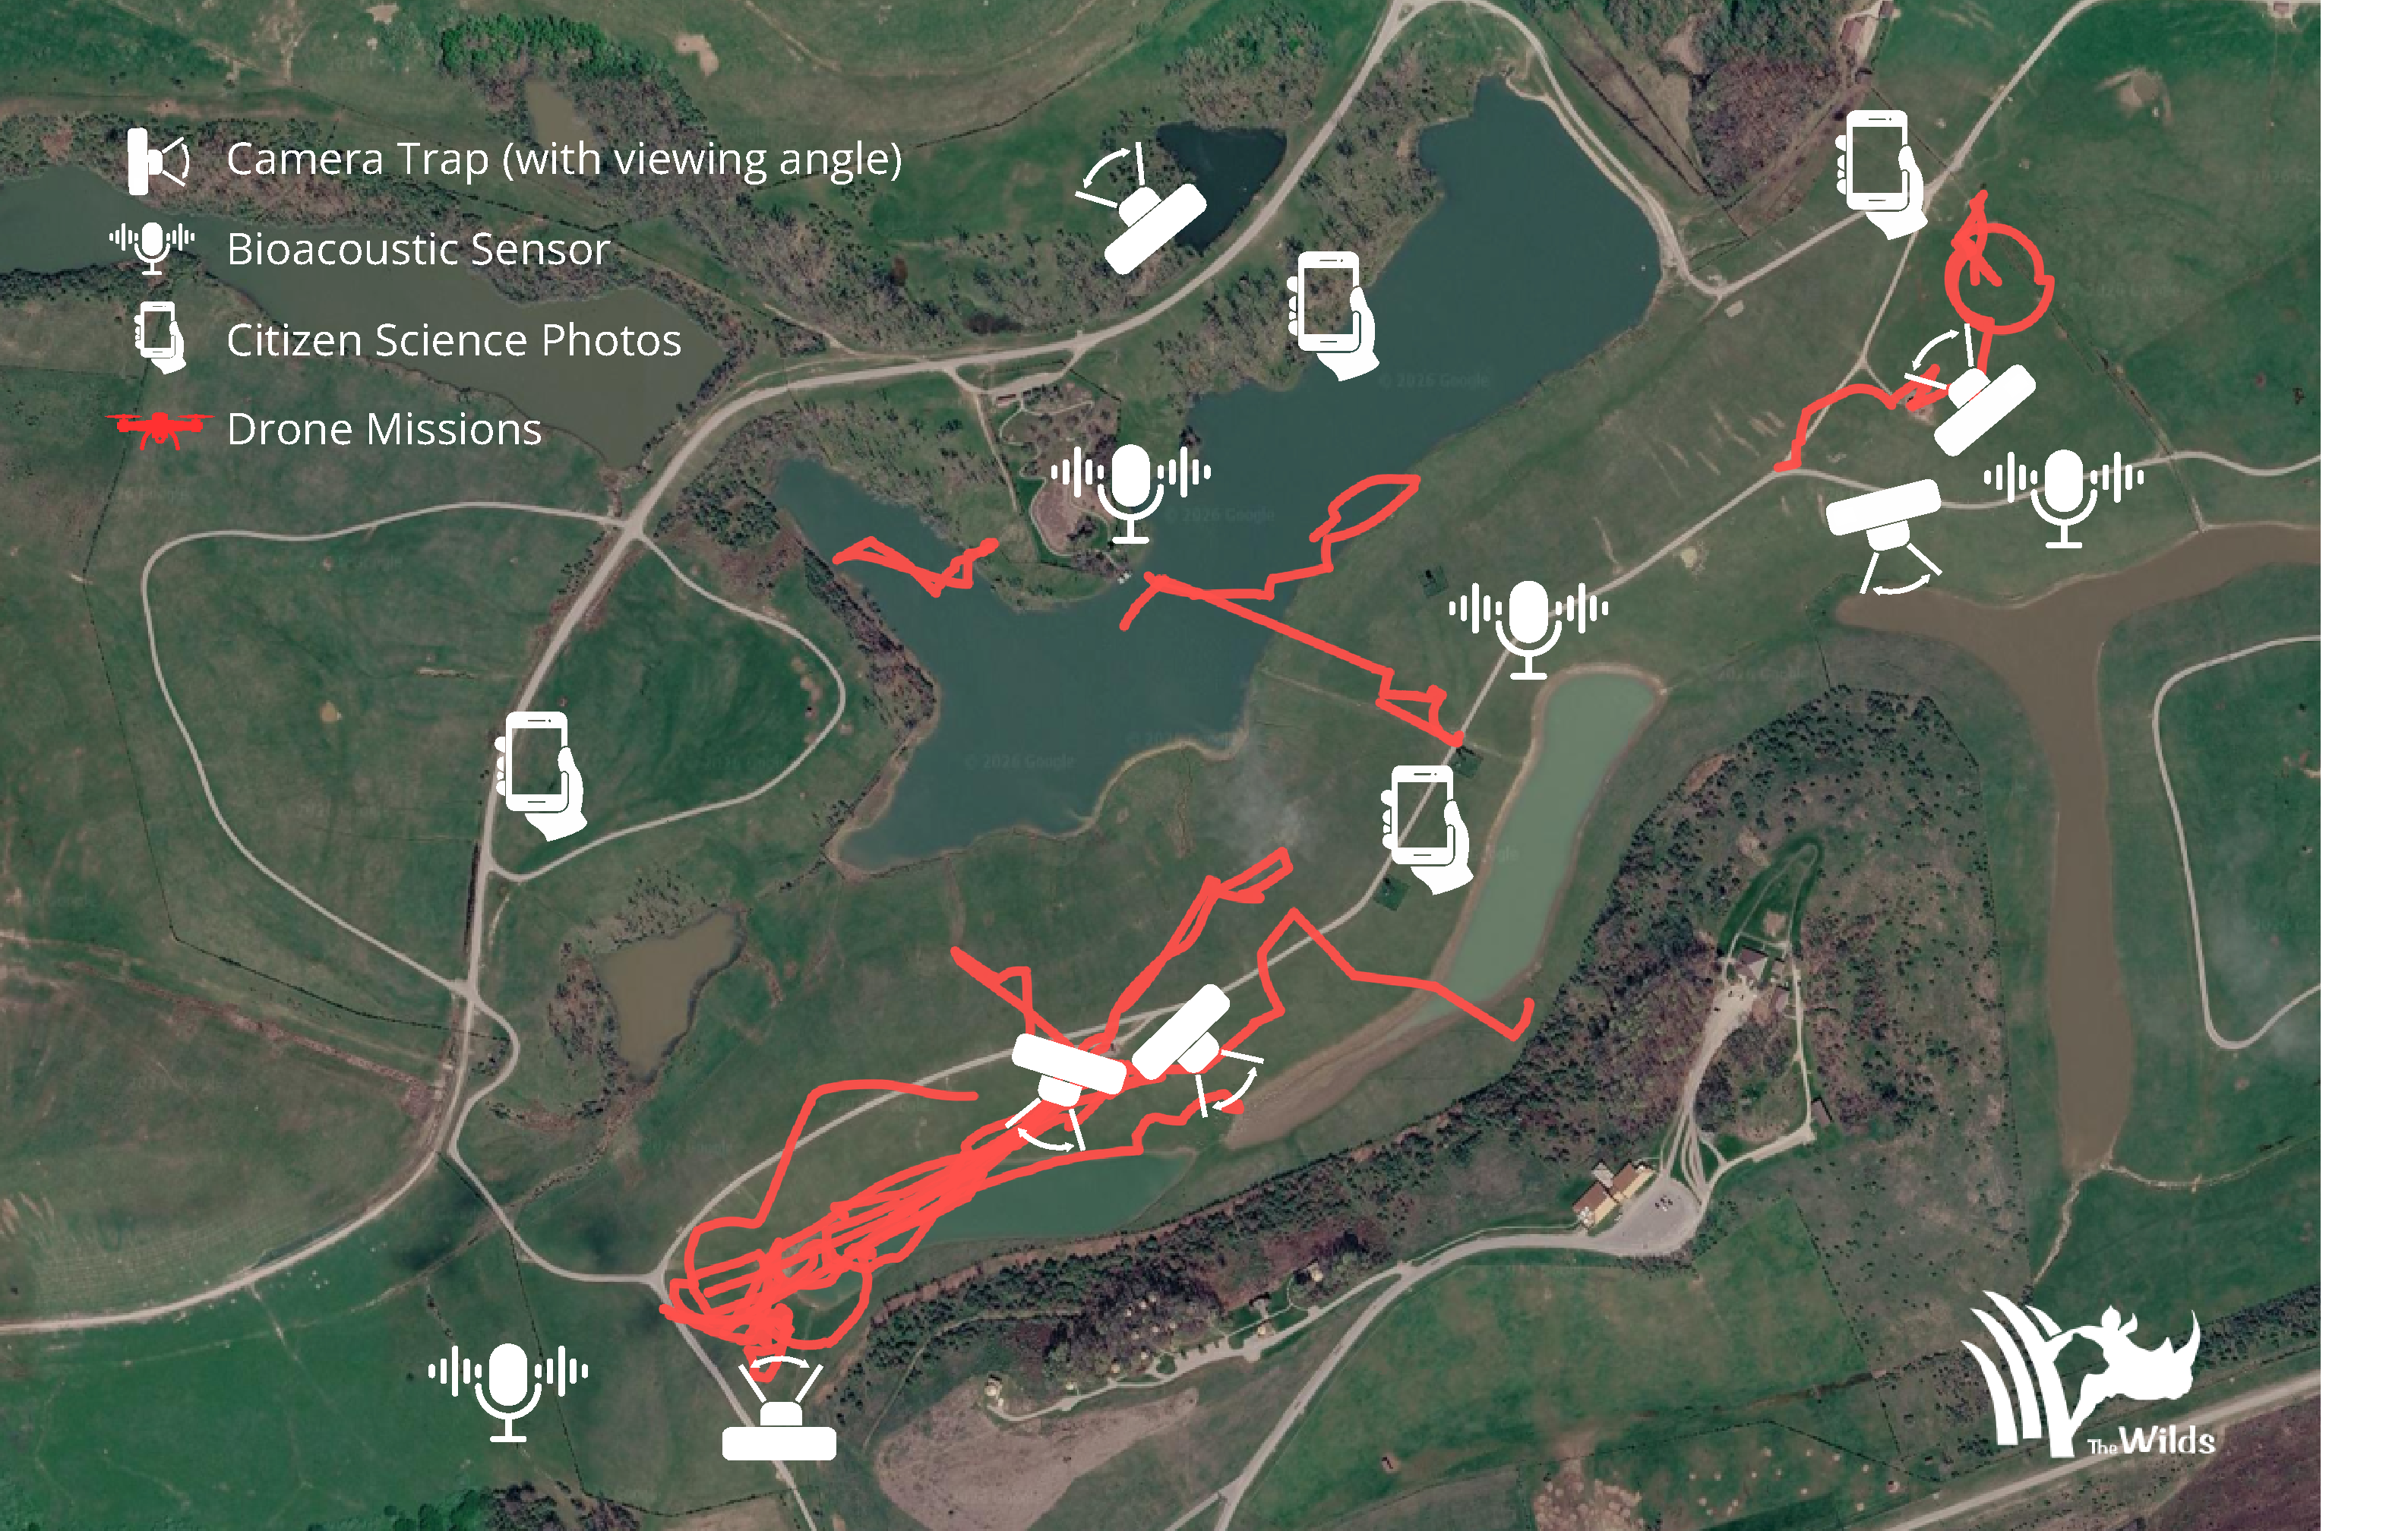
\includegraphics[width=\linewidth]{figures/smartwildsmap.pdf}
        \caption{Sensor deployment across the study area: camera traps
        with viewing angles, Song Meter recorders, citizen-science
        localities, and drone flight tracks (red). Satellite imagery
        \copyright\ Google.}
        \label{fig:map}
    \end{subfigure}\hfill
    \begin{subfigure}[b]{0.51\textwidth}
        \centering
        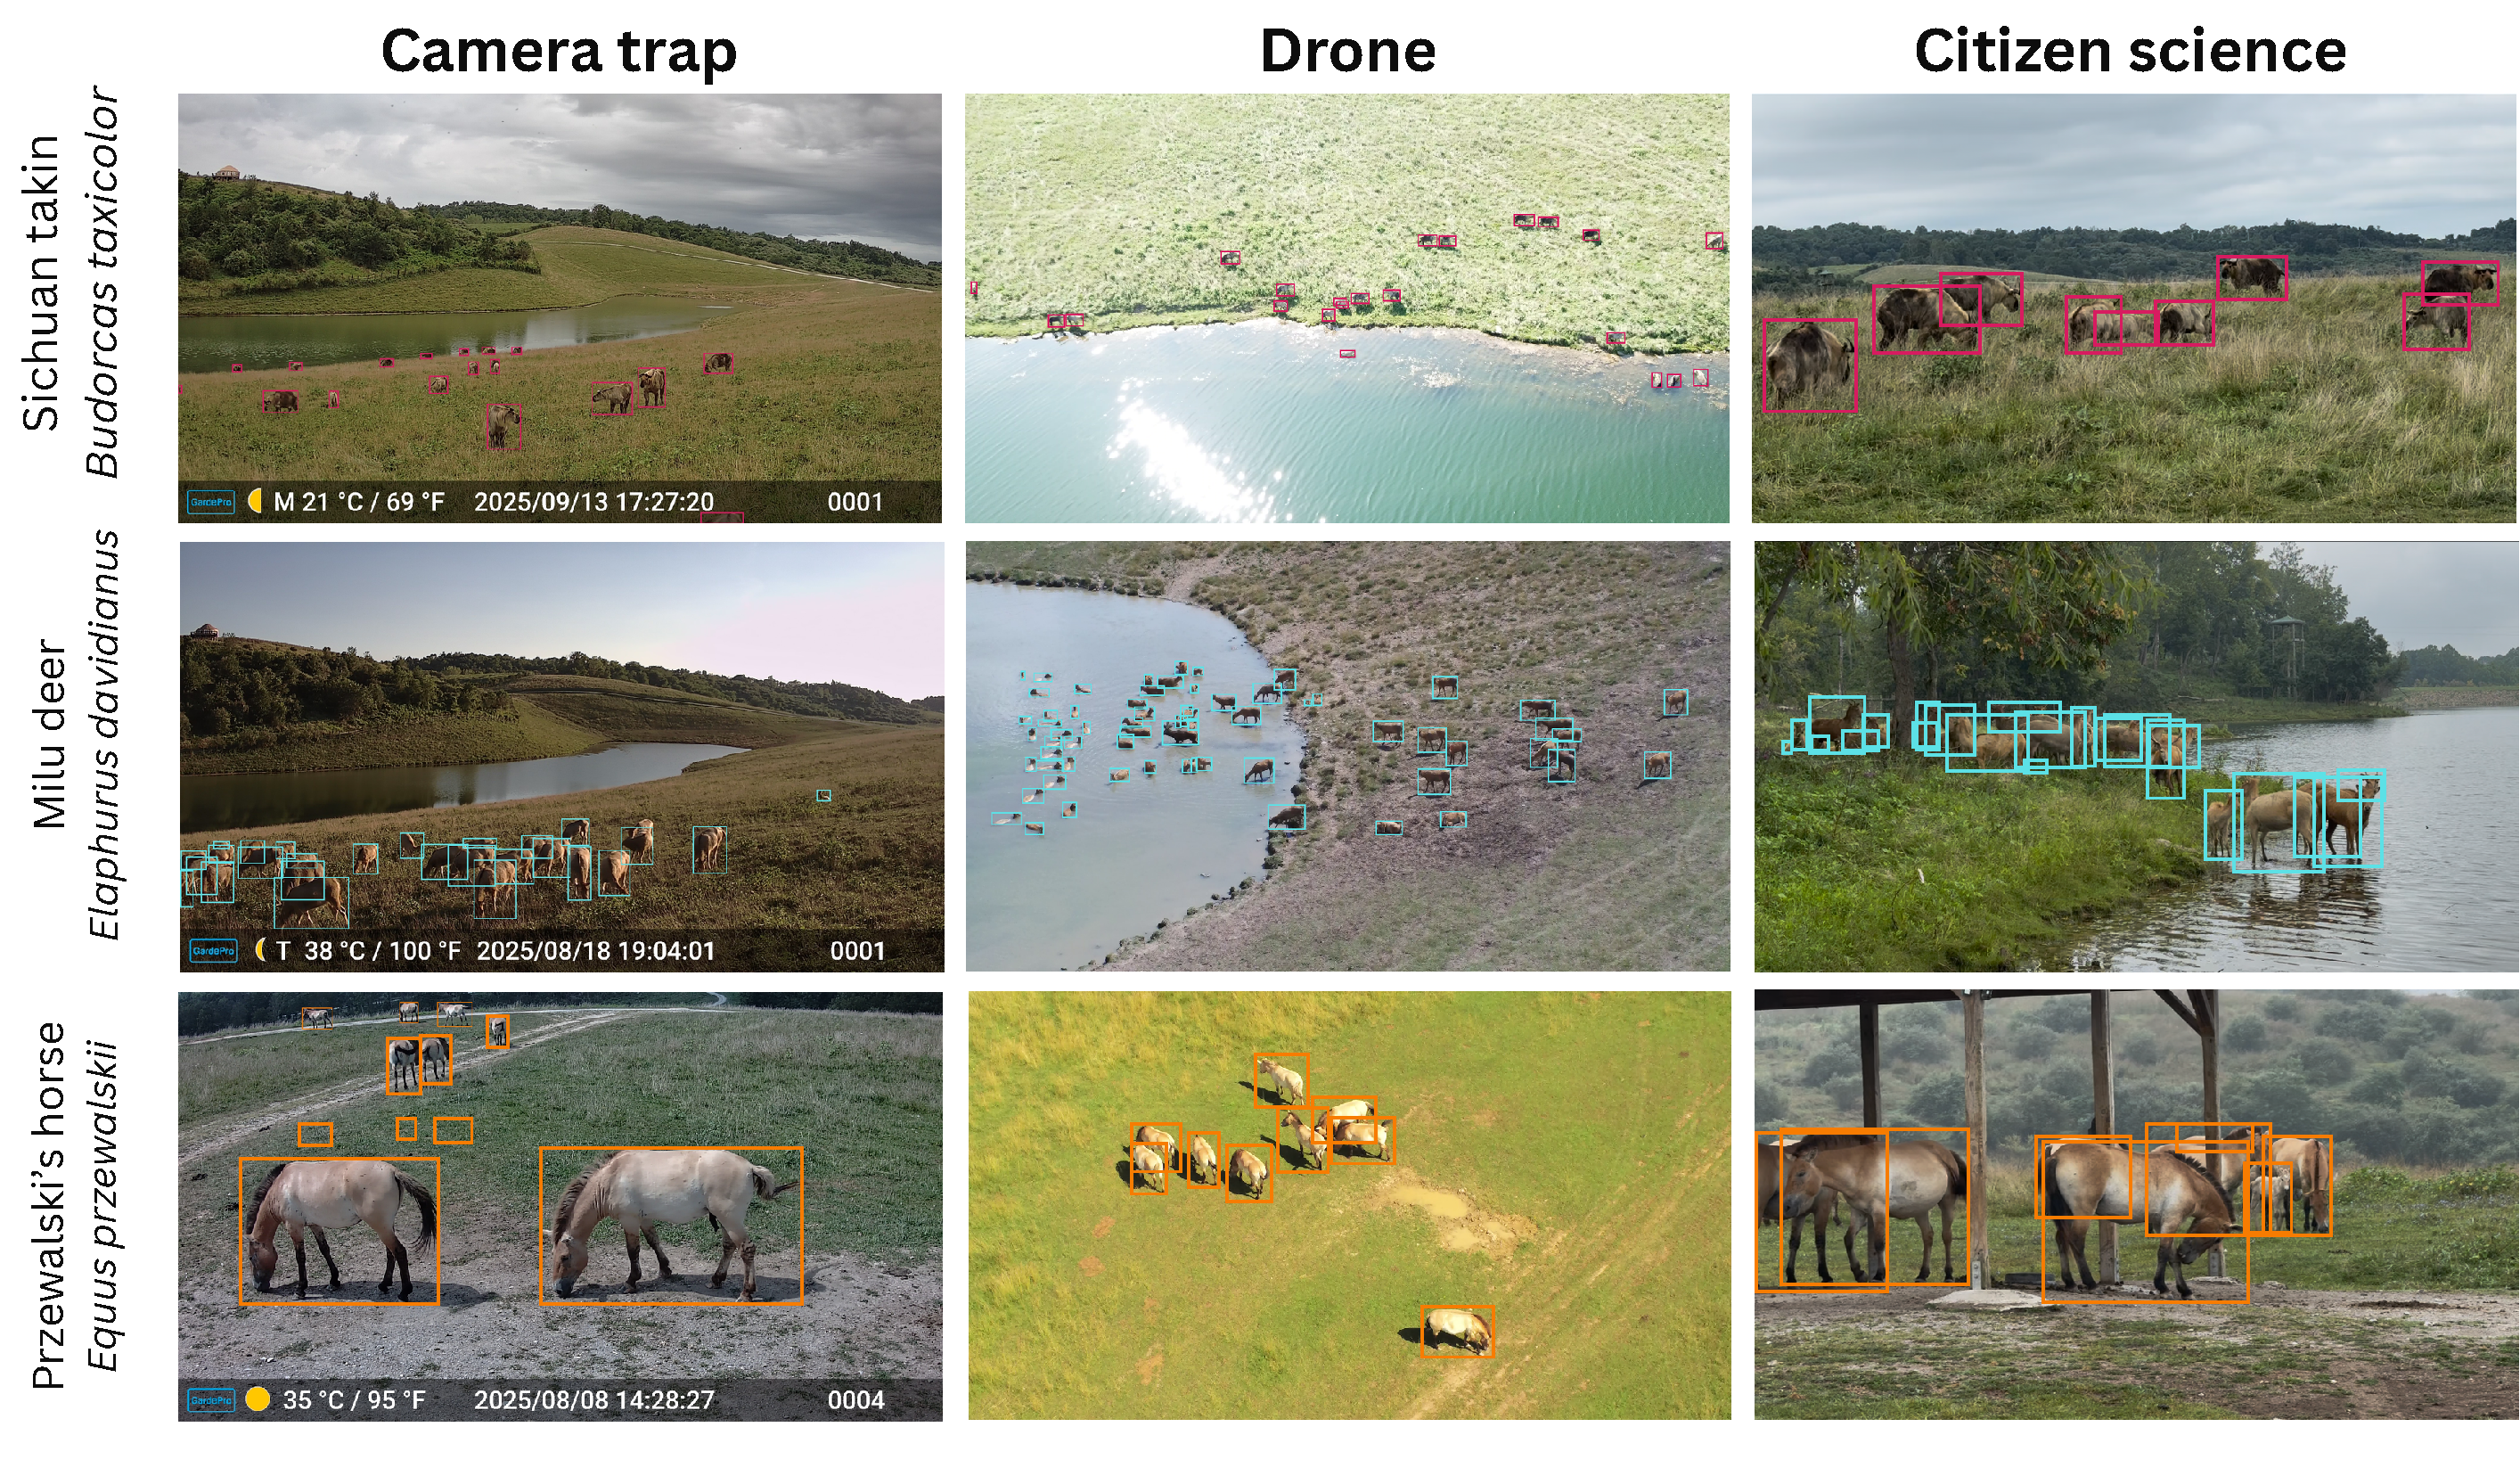
\includegraphics[width=\linewidth]{figures/datapreview.pdf}
        \caption{The same three managed focal species (Sichuan takin,
        Milu deer, Przewalski's horse) seen by camera trap, drone, and
        citizen science, with SAM3 detections. Camera overlays show the
        raw device clock (the takin frame reads 2025/09/13 for an August
        image; \S\ref{sec:timestamps}).}
        \label{fig:preview}
    \end{subfigure}
    \caption{The \smartwilds modalities differ in spatial support as
    well as cadence: cameras and recorders sample fixed points, drones
    sweep the pastures and lake margin, and citizen-science records
    resolve only to a locality (a); and they differ in viewpoint, scale,
    and resolution for the same animals (b).}
    \label{fig:overview}
\end{figure*}

\subsection{Data Collection Campaign}

Data collection comprised three campaigns (Table~\ref{tab:campaigns}):
a four-day pilot (2025-06-30 to 07-03) that established site selection,
mounting, and configuration practice; the main deployment
(2025-08-04 to 08-28), a 24-day span over 25 calendar dates with all
four modalities, nine camera installations, six recorder deployments,
and drone flights on three dates; and a single-day drone revisit
(2025-09-08) with a different platform. All characterization in
\S\ref{sec:characterization} uses Campaign~2, the only window in which
all modalities were simultaneously active.

\begin{table}[t]
\caption{Campaign structure and raw data volume. Volumes are
on-disk sizes in the project archive.}
\label{tab:campaigns}
\small
\begin{tabular}{llrrr}
\toprule
& & \textbf{C1} & \textbf{C2} & \textbf{C3} \\
\midrule
\multicolumn{2}{l}{Start} & 2025-06-30 & 2025-08-04 & 2025-09-08 \\
\multicolumn{2}{l}{End} & 2025-07-03 & 2025-08-28 & 2025-09-08 \\
\multicolumn{2}{l}{Calendar dates} & 4 & 25 & 1 \\
\midrule
\multirow{2}{*}{Camera traps} & GB & 49 & 211 & --- \\
 & files & 20{,}027 & 220{,}898 & --- \\
\multirow{2}{*}{Bioacoustics} & GB & 6.0 & 196 & --- \\
 & files & 318 & 2{,}157 & --- \\
\multirow{2}{*}{Drones} & GB & 46 & 33 & 11 \\
 & files & 35 & 20 & 22 \\
\multirow{2}{*}{Citizen science} & GB & --- & 9.4 & --- \\
 & files & --- & 1{,}103 & --- \\
\midrule
\multicolumn{2}{l}{\textbf{Total (GB)}} & \textbf{101} & \textbf{449} & \textbf{11} \\
\bottomrule
\end{tabular}
\end{table}

\subsection{Sensing Modalities and Configurations}

We deployed deliberately \emph{heterogeneous} hardware. The resulting
configuration diversity is the largest single source of downstream
metadata work, and it is why the configuration tables are part of the
release.


\subsubsection{Camera traps}
Thirteen deployments used four camera models with horizontal fields of
view from 55$^\circ$ to 120$^\circ$, varying in capture mode (photo-only,
photo+video, hybrid with hourly timelapse), resolution (4\,MP, 8\,MP,
4K), burst length (3 or 5 frames per trigger), PIR sensitivity, and
inter-trigger delay (0--20\,s). One model is cellular-capable, making it
the only device here that could in principle participate in
near-real-time coordination.

Each parameter is a workload multiplier: a 5-frame burst produces five
times the raw images per ecological event as a single capture, a 20\,s
delay suppresses repeat triggers and lowers the effective arrival rate,
and video mode adds a 10--15\,s clip per trigger with disproportionate
storage and frame-extraction cost. The 13 deployments yielded
235{,}778 still images and 5{,}113 video clips, distributed extremely
unevenly: one dock-facing deployment produced 90{,}834 images, 38.5\% of
the total, while four produced fewer than 100 each. Per-deployment
models, configurations, and counts are in the supplement.



\subsubsection{Bioacoustics}
All acoustic recording used Wildlife Acoustics Song Meter Micro 2 units
at 48\,kHz. Ten deployments across six sites produced 2{,}453 WAV files.
Duty cycles differed deliberately: 5\,min/hour (8.3\%), 15\,min/hour
(25\%), continuous sunrise-to-sunset (roughly 50--60\% seasonally), and
continuous 24/7. One Campaign~1 unit was misconfigured --- intended to
record one hour at sunrise and sunset, it instead recorded 5-minute
clips hourly --- an error we discovered only from the resulting file
inventory.

Duty cycle dominates acoustic storage, since uncompressed 48\,kHz stereo
WAV runs roughly 33\,MB/minute. The two sunrise-to-sunset units each
produced over 56\,GB in 24 days, while the 5\,min/hour unit produced
26\,GB from more than twice as many files --- file count and byte volume
are independent axes. Per-deployment schedules, GPS positions, and
counts are in the supplement.



\subsubsection{Drones}
Drone survey used three platforms: a Parrot Anafi 4K (10 video-bearing
sessions across both campaigns; three additional Aug.~25 directories contained
metadata but no video; 4K MP4 video with Parrot JSON / GUTMA DX telemetry),
an unspecified DJI airframe (one Campaign~2 session,
1080p MOV with 10\,Hz CSV telemetry), and a DJI Air 2 (four Campaign~3
flights, 4K MP4 with Airdata CSV telemetry). The three platforms
produced three telemetry schemas with different field names, units
(feet vs.\ meters for altitude), and gimbal-angle conventions ---
a reconciliation cost documented in \S\ref{sec:scope}.

\subsubsection{Citizen science and text records}
Park visitors submitted photographs and observations through a
structured web form, yielding 1{,}103 raw-folder media files. Manual annotation
covered 791 photos and retained 564 wildlife photos, which yield 622 taxon
Occurrences; 50 curated September 8 photos are Google Photos album-export assets
outside the raw folder. Visitor submissions arrive only within operating hours,
producing the sharply truncated
diurnal profile in \S\ref{sec:characterization}. We additionally
curated a small set of text-derived records from field notes and
site-selection rationale, which we retain as a distinct modality
because they carry the human reasoning behind sensor placement.

\subsection{Field Protocol and Human Workflow}

Each cycle involved site selection, mounting and configuration,
periodic servicing, SD-card retrieval, transfer to institutional
storage, and logging. Two structured field logs, camera-trap and
bioacoustic, were captured through forms during Campaign~2; they are the
metadata most relied on in the release (\S\ref{sec:redundancy}). Human effort concentrated in two places: SD-card handling, where one camera's data arrived split
across several cards with inconsistent clock states, and the timestamp
reconstruction of \S\ref{sec:timestamps}.

\subsection{Ethics, Permissions, and Sensitive Records}

All work was conducted with the permission and participation of The
Wilds. Two categories of sensitive content required handling. Visitor
imagery: the TW07-CT05 deployment captured only people on tour buses and
no wildlife. Its deployment note states that the camera was monitored
through the mobile app and that the people-only photos were not uploaded;
the release contains no image, Event, or Occurrence from this deployment.
The retained archive holds only metadata for this deployment; whether
images on the device were later deleted is not recorded. And locality precision: citizen-science
coordinates are generalized and records for sensitive taxa are reduced
in precision via Darwin Core \texttt{informationWithheld} and
\texttt{dataGeneralizations}.

% ============================================================
\section{Data Model}
\label{sec:model}

The data model has three jobs. It keeps the release \emph{ecologically
grounded}: records are Darwin Core Events and Occurrences whose
taxonomy, sampling protocol, and effort terms biodiversity
infrastructure such as GBIF already consumes. It supports
\emph{cross-modal coordination}: all modalities share one Event
hierarchy, one corrected time base, and typed spatial semantics, so a
query over a time window or site returns observations from every sensor,
and a trigger from one modality to another can be evaluated against the
record. And it carries the \emph{operational metadata} --- schedules,
trigger settings, clock and coordinate provenance, model identity, and
typed missingness --- that ecological and computer-vision releases
discard.

\subsection{Terminology}
\label{sec:glossary}

Ecology, computer vision, and sensing systems overload the same small
set of words, and in a cross-modal release that ambiguity is a direct
source of analysis error; supplement S1 fixes our full vocabulary.
The entry that matters most is \emph{Event}: in Darwin Core a sampling
act with a location, date, and
protocol~\cite{wieczorek2012darwincore,tdwgDarwinCore}; in sensing
systems an arrival in a stream. They are not in correspondence --- one
Darwin Core Event, a 24-day camera deployment, contains tens of
thousands of image captures. We keep the Darwin Core meaning for the
record types we release and the FAIR\textsuperscript{2} Drones
conventions for effort and platform
metadata~\cite{pierrat2025proximal}, and say \emph{arrival} for the
systems sense.


\subsection{Design Requirements}

The model serves two audiences: ecologists want Darwin Core records they
can push to GBIF, systems researchers want device schedules, trigger
semantics, and failure records. Rather than maintain two releases we use
Darwin Core as the interchange layer and extend it, keeping every
systems field in a named column rather than in prose. Six requirements
drove the design --- \emph{ecological grounding}, so every record is
valid Darwin Core with standard taxonomy, protocol, and effort terms;
\emph{cross-modal alignment}, so observations from any modality join
on a shared Event root, corrected time, and typed location;
\emph{heterogeneity}, so fixed sensors and moving
platforms are first-class rather than special cases of each other;
\emph{traceability}, so every Occurrence resolves to a device, a time
reference, a spatial reference, and a transformation chain;
\emph{explicit uncertainty}, so estimated quantities are distinguishable
from observed ones per record rather than per dataset; and
\emph{extensibility}, so a fifth modality does not require re-keying the
first four.

\subsection{Four-Level Event Hierarchy}

Events form a four-level tree (Figure~\ref{fig:hierarchy}):

\begin{description}
\item[Study.] One root event, \texttt{TheWilds\_2025}, spanning the full
campaign extent (2025-06-30 to 2025-09-08) with a coarse study-area
coordinate and 5\,km uncertainty.
\item[Project.] One per modality (camera traps, bioacoustics, drones,
citizen science, text data), carrying the modality's sampling protocol
and aggregate sample size.
\item[Deployment / session.] One per physical installation or mission:
\texttt{SensorDeployment} for the 12 retained camera installations and
10 recorder deployments, and for the 15 video-bearing drone flight sessions. These
carry fixed coordinates (5\,m uncertainty) for stationary sensors,
device model and serial, schedule, and deploy/retrieve dates.
\item[Capture.] One per acquisition unit below the deployment:
2{,}371 \texttt{AudioRecording} events (one per processed WAV file,
with start time and duration, including 64 recordings on which BirdNET
emitted no detection), 39 \texttt{MediaEvent} events (one per raw drone
video, including one reviewed and excluded video with no Occurrences),
and 17 \texttt{ObservationSession} events for citizen-science and text
records.
\end{description}

The resulting table holds 2{,}470 Darwin Core Events
(Table~\ref{tab:schema}). Occurrences attach to the lowest available
level via \texttt{eventID}, so an acoustic detection resolves to a
specific WAV file while a camera-trap detection resolves to a deployment
interval.
\TODO{Post-triage camera Occurrences attach to per-image \texttt{Image}
Events; update this sentence and the hierarchy description once those
Events are merged into the release table.} The asymmetry is deliberate: flattening it would fabricate
acquisition-boundary precision the cameras do not provide.

\begin{table}[t]
\caption{Darwin Core Event hierarchy and Occurrence counts in the
released snapshot (\texttt{darwin\_core\_\allowbreak latest\_\allowbreak 20261008}). Hourly bins count
distinct (date, hour) pairs containing at least one Occurrence, over
the full study extent (2025-06-30 to 2025-09-08). The 2025-08-11 drone
session carries a date but no time (\S\ref{sec:nulldefect}), so it
counts toward drone dates but not bins.
\TODO{Camera dates/bins (29 / 624) assume the 439 curated camera
Occurrences are re-timed from the corrected timestamp map; the current
snapshot gives 30 / 625.}
\TODO{Camera row and totals predate the post-triage camera tables
(72{,}769 Occurrences; 1 Project + 12 SensorDeployment + 19{,}749
Image Events). Update after the merged snapshot is regenerated; the
same totals (552{,}964 Occurrences, 2{,}470 Events) appear in the
abstract, contributions, \S\ref{sec:using}, and the conclusion.}}
\label{tab:schema}
\small
\begin{tabular}{lrrrr}
\toprule
\textbf{Modality} & \textbf{Events} & \textbf{Occ.} & \textbf{Dates} & \textbf{Bins} \\
\midrule
Study root & 1 & --- & & \\
Camera traps & 13 & 224{,}149 & 29 & 624 \\
Bioacoustics & 2{,}382 & 9{,}960 & 29 & 650 \\
Drones & 55 & 318{,}203 & 6 & 8 \\
Citizen science & 14 & 622 & 13 & 28 \\
Text data & 5 & 30 & 4 & 4 \\
\midrule
\textbf{Total} & \textbf{2{,}470} & \textbf{552{,}964} & & \\
\bottomrule
\end{tabular}
\end{table}

\begin{figure}[t]
    \centering
    \resizebox{\linewidth}{!}{% SmartWilds release schema (ER-style). Darwin Core core tables: dark headers.
% SmartWilds extension tables: light headers. Arrows point from FK to PK.
\begin{tikzpicture}[
  font=\scriptsize,
  tbl/.style={draw, rectangle split, rectangle split parts=2,
              rectangle split part fill={#1,white}, inner sep=2pt,
              align=left, rounded corners=1pt},
  core/.style={tbl=black!75, text width=3.75cm},
  ext/.style={tbl=black!15, text width=3.45cm},
  fk/.style={-{Latex[length=1.5mm]}, semithick},
  lbl/.style={font=\tiny\itshape, inner sep=0.8pt},
]
\newcommand{\pk}[1]{\underline{#1}}
% ---------------- Darwin Core core (left column) ----------------
\node[core] (ev) at (0,0) {\textcolor{white}{\textbf{Event}\hfill 2{,}470 rows}
  \nodepart{two}\raggedright
  \pk{eventID}\\
  parentEventID $\rightarrow$ Event\\
  eventType (4 levels)\\
  eventDate, eventTime\\
  lat, lon, uncertainty\\
  samplingProtocol, sampleSize\\
  fieldNotes (provenance)};
\node[core, below=4mm of ev] (oc) {\textcolor{white}{\textbf{Occurrence}\hfill 552{,}964 rows}
  \nodepart{two}\raggedright
  \pk{occurrenceID}\\
  eventID $\rightarrow$ Event\\
  taxon ranks, basisOfRecord\\
  identifiedBy (model, version)\\
  verificationStatus\\
  remarks: score, box, status\\
  coordinates + generalization\\
  associatedMedia $\rightarrow$ Media};
\node[ext, below=4mm of oc] (arr) {\textbf{Arrival traces}
  \nodepart{two}\raggedright
  sourceID $\rightarrow$ Occ. $|$ Event\\
  layer, timestamp, eligibility};
% ---------------- SmartWilds extensions (right column) ----------------
\node[ext, anchor=north west] (dep) at ([xshift=6mm]ev.north east) {\textbf{Deployment settings}
  \nodepart{two}\raggedright
  deploymentID $\rightarrow$ Event\\
  model, HFOV, bearing\\
  schedule, trigger, burst};
\node[ext, below=2.5mm of dep] (rec) {\textbf{WAV reconciliation}
  \nodepart{two}\raggedright
  eventID $\rightarrow$ Event\\
  path, status, disposition};
\node[ext, anchor=north west] (det) at ([xshift=6mm, yshift=-1mm]oc.north east) {\textbf{Drone detections}
  \nodepart{two}\raggedright
  occurrenceID $\rightarrow$ Occ.\\
  video, frame\_index, box};
\node[ext, below=2.5mm of det] (med) {\textbf{Media manifest}
  \nodepart{two}\raggedright
  \pk{release\_path}\\
  bytes, include flag\\
  exclusion reason\\
  has\_human\_detection};
\node[ext, below=2.5mm of med] (img) {\textbf{Image timestamps}
  \nodepart{two}\raggedright
  release\_path $\rightarrow$ Media\\
  raw ts + source\\
  corrected ts, method\\
  confidence};
% ---------------- relationships (FK -> PK) ----------------
\draw[fk] ([yshift=-1.5mm]ev.two west) -- ++(-3mm,0) |- node[lbl, left, pos=0.25] {self} ([yshift=1.5mm]ev.text west);
\draw[fk] (oc.north) -- (ev.south);
\draw[fk] (arr.north) -- (oc.south);
\draw[fk] (dep.west) -- (dep.west -| ev.east);
\draw[fk] (rec.west) -- (rec.west -| ev.east);
\draw[fk] (det.west) -- (det.west -| oc.east);
\draw[fk] (med.west -| oc.east) -- node[lbl, above] {media} (med.west);
\draw[fk] (img.north) -- (med.south);
\end{tikzpicture}
}
    \caption{Release schema. Darwin Core core tables (dark) and
    \smartwilds extension tables (light); arrows run from foreign key to
    primary key. The Event table is self-referencing and encodes the
    four-level hierarchy (study $\supset$ modality project $\supset$
    deployment or session $\supset$ capture), so fixed sensors and moving
    platforms both sit at the deployment level and a cross-modal query
    over a time window returns both without special-casing. Extension
    tables carry what Darwin Core cannot: sensor settings, timestamp
    provenance, media inclusion and privacy status, frame-level drone
    detections, per-file acoustic disposition, and versioned arrivals.}
    \label{fig:hierarchy}
\end{figure}

\subsection{Identifiers and Spatial Semantics}
\label{sec:identifiers}

Identifiers encode what kind of thing they name: fixed sensor
deployments use \texttt{TW\{site\}-\{device\}\_\{start\}\_\{end\}},
drone sessions \texttt{\{date\}\_\{platform\}\_\{seq\}}, and capture
Events append the acquisition identifier --- a convention that also
proved error-correcting (\S\ref{sec:nulldefect}).
\texttt{locationID} is populated \emph{only} for fixed sensor sites
(7 camera, 6 recorder) and drone session origins (15); citizen-science
records carry a locality name and a null \texttt{locationID}. This is the most consequential typing decision in
the schema: a \texttt{GROUP BY locationID} cannot present 15 drone
session origins and 7 fixed camera positions as comparable sampling
units, because the semantics are documented per modality and the
locality-only rows are null rather than coerced.

Spatial support differs by modality and is recorded as such.
Deployment-level coordinates are sensor positions with 5\,m uncertainty.
Occurrence-level coordinates are estimated animal or platform
positions for drones, recorder positions for acoustics, and generalized
localities for citizen science. Each carries a coordinate
uncertainty (\texttt{coordinate\allowbreak Uncertainty\allowbreak InMeters})
and a \texttt{data\allowbreak Generalizations} string saying which it is; camera
Occurrences carry no coordinate of their own and inherit the deployment
position.

\subsection{Semi-Automated Labels and Model Provenance}
\label{sec:provenance}
\label{sec:modelprov}

Data volume grows with device count and duty cycle while expert review
capacity does not, so labels are produced by current models and human
review is spent where it changes the most labels.
\emph{Camera-trap} Occurrences are SAM3~\cite{carion2026sam} animal
proposals labeled by embedding-based triage: the triage selects
proposals for human review and resolves the remainder by similarity to
reviewed examples. Of 72{,}769 retained boxes across 12 taxa, 1{,}760
labels are human-reviewed, 70{,}808 machine-resolved, and 201 forced
nearest-neighbour assignments that did not meet the triage confidence
rules. The Occurrence table excludes boxes with a shorter side below
32\,px or overlapping a per-resolution ROI mask, so an image without an
Occurrence is not an observed absence. \emph{Drone} Occurrences pair a
SAM3 box with a top-1 BioCLIP
Tree-of-Life~\cite{stevens2024bioclip,gu2025bioclip,treeoflife_200m}
taxon and its full rank hierarchy, plus a projected ground coordinate
where telemetry permits (\S\ref{sec:scope}). \emph{Acoustic}
Occurrences are BirdNET~\cite{kahl2021birdnet} detections with an
offset into the source WAV. Following scientific-workflow provenance
practice~\cite{simmhan2005provenance}, the chain from raw asset through
model to Occurrence is recorded per record, with scripts and
configurations released beside the data.

When labels are model outputs, the model is part of the data. A taxon
string is reproducible only with the model identity, version, and
inference parameters that produced it, and a release that keeps source
media, detection geometry, and label provenance can be
\emph{re-labeled} as models improve. Each camera Occurrence records
whether its label was reviewed, resolved, or forced
(\texttt{labelProvenance}, with the triage round) and that its geometry
is the unedited SAM3 proposal. A separate reference set of 2{,}067
human-reviewed boxes on 198 camera images --- ungulates and waterfowl,
including edited and added boxes --- is kept out of the Occurrence
table and supports evaluation. SAM3 localization on a human-annotated
camera-trap subset reaches F1 0.856 at IoU $\geq 0.50$ ($n{=}1{,}125$).
BioCLIP accuracy falls with rank, from 0.845 at class to 0.271 at
species ($n{=}951$), so drone labels support screening at class rank and
require curation at species rank. Verification status is carried per
record, so a verification floor is a single predicate over the release.
\TODO{Report triage label accuracy against the reference set (or cite
the WACV paper's figures); recount
\texttt{identificationVerificationStatus} across modalities --- the
previous partition (550{,}722 / 1{,}590 / 652) assumed the BioCLIP
camera labels.}

\subsection{Missingness as Data}

The schema distinguishes six states that would otherwise collapse into a
single absence:

\emph{(1) Sensor active, nothing observed}, recoverable from the
deployment interval and schedule: an hourly bin inside a deployment
window with no Occurrence means the sensor was on and did not detect.
\emph{(2) Sensor inactive by schedule} --- the 5\,min/hour recorders are
off 91.7\% of the time by design, which the deployment-level schedule
field makes computable, as acquisitional sensor
databases require~\cite{madden2005tinydb}. \emph{(3) Sensor inactive by failure}, such as
battery exhaustion at TW02-CT01 (Aug 18--25), recorded as a gap with a
cause. \emph{(4) Captured but not represented}: of 2{,}453 WAV paths on
disk, 2{,}371 are \texttt{AudioRecording} Events; 78 are Campaign-1
files copied into a Campaign-2 directory during transfer and are
duplicates rather than recordings, and 4 produced no BirdNET result
(three 3.9--22.0\,s fragments and one unreadable file). A one-row-per-path
reconciliation table records the class of every file, and 64 processed
recordings with zero detections are retained as Events with no
Occurrences, so ``processed, nothing heard'' is distinguishable from
``not processed''.
\emph{(5) Metadata unusable for a purpose}: 41{,}524 drone Occurrences
(13.1\%) carry a date recovered from their identifier but no time of
day (\S\ref{sec:nulldefect}), and separately
70{,}219 detections cannot support per-animal ground projection and
retain platform coordinates with a status code (\S\ref{sec:scope}) ---
adequate for the campaign's purpose, unusable for one it was not
collected for. \emph{(6) Excluded in QC}: the people-only TW07-CT05
deployment is excluded and documented as such, so its absence does not
read as a site with no wildlife; one drone video, reviewed and found to
contain no usable content, is retained as a \texttt{MediaEvent} with no
Occurrences for the same reason.

States (1) and (2) have opposite implications for a coordination policy,
which is why the schedule field is required rather than descriptive.

\subsection{Standards Alignment}
\label{sec:crosswalk}

Darwin Core and its Humboldt extension~\cite{tdwgHumboldt} cover
taxonomic and Event structure well, and we reuse them directly for
taxon, date, coordinate, uncertainty, verification status, and effort
terms. We adopt the FAIR\textsuperscript{2} Drones card as the
documentation template~\cite{pierrat2025proximal}, express device
specifications in the spirit of SensorML~\cite{ogcSensorML} and
derivation in the spirit of PROV-DM~\cite{w3cProvDM} without encoding
either, and follow FAIR, CARE, and TRUST for
release~\cite{wilkinson2016fair,carroll2020care,lin2020trust}.

Six classes of information required for cross-modal reuse are
expressed by no standard we found in a machine-readable way: per-device
duty cycle and acquisition schedule; trigger semantics such as PIR
sensitivity, burst length, and inter-trigger delay; timestamp confidence
and repair method; per-detection coordinate provenance status; typed
missingness; and model identity with per-rank accuracy. We have named
these, used them consistently across modalities, and documented them
in the full crosswalk in the supplement.

% ============================================================
\section{Quality Control}
\label{sec:qc}

We encountered 20 defect classes. Table~\ref{tab:defects} groups them
by what each was \textbf{detected by}, because that is what determined
whether we could repair it; the full per-class inventory, with scope,
repair, and residual risk, ships with the release.

Clock error, battery failure, misconfiguration, and media
fragmentation are documented hazards of camera-trap and recorder
deployment~\cite{lahozmonfort2021monitoring,ahumada2020wildlifeinsights,Pestell2025SmartCamera}.
We organize the inventory by detection
source because detectability, rather than device reliability, is what
separated the repairable defects from the permanent ones; the release
inventory quantifies both the repairs and the residual uncertainty.

\begin{table}[t]
\caption{Defect classes by what made them detectable. All 20 classes,
with scope, repair, and residual risk, are inventoried in the release
(\texttt{metadata/DEFECT\_INVENTORY.md}) and supplement~S16.}
\label{tab:defects}
\small
\begin{tabular}{p{0.36\linewidth}rp{0.38\linewidth}}
\toprule
\textbf{Detected by} & \textbf{Classes} & \textbf{Example} \\
\midrule
External record (service log, field note, platform docs) & 5 & Wrong or unset camera clocks (93.9\% of images) \\
Redundant encoding in the data & 2 & \texttt{nan} date recovered from the \texttt{eventID} \\
Cross-check between artifacts & 8 & 146 WAV files with no \texttt{AudioRecording} Event \\
Human inspection & 3 & Visitor-only camera deployment \\
\midrule
None (fact recorded once) & 2 & Within-card clock drift \\
\bottomrule
\end{tabular}
\end{table}

\subsection{Detectability and Redundancy}
\label{sec:redundancy}

Eighteen of the twenty defect classes (Table~\ref{tab:defects}) were
repairable, and in every case the repair was possible because the fact
the device got wrong had been recorded somewhere a second time. The
general property is \emph{redundancy} rather than independence: two of
the six sources below sit inside the data the pipeline itself produced,
and they worked as well as the external ones. The six fall into four
families --- records external to the device, redundant encodings within
the data, cross-checks between two artifacts, and human inspection ---
and all six are cheap to produce at deployment time:

\begin{description}
\item[Service and deployment logs.] Two structured field logs from
Campaign~2 record when each device was deployed, serviced, and
retrieved --- the sole reason the clock defects were repairable, since a
camera asserting 2023 is correctable only against an external claim
about when it was in the field. Cost: minutes per visit.

\item[Field notes on deployment changes.] A free-text note that
TW09-CT02 moved from the dock to Nomad Ridge W on Aug 18 turned
90{,}834 images from one mislocated block into two correctly located
intervals; nothing in the device's output indicated the move. Cost: one
sentence.

\item[Cross-checks.] Comparing disk against pipeline output caught the
misconfigured recorder schedule, 146 unrepresented WAV files, and an
unprocessed drone video --- free, but only if raw media are retained
beside derived products.

\item[Redundancy in device output.] Three camera models burn the
timestamp into the image. For 182 images with no surviving filename or
EXIF timestamp, that pixel-level duplicate was the only record,
recoverable by OCR. This is the lowest-cost redundancy in the
deployment, and the vendor rather than the field team supplied it.

\item[Redundancy in identifiers.] Our \texttt{eventID}
convention embeds the acquisition date. When an entire drone session's
\texttt{eventDate} was written as the string \texttt{nan}, the
identifier was the only surviving record of when the flight happened
(\S\ref{sec:nulldefect}). The convention, adopted for readability,
also provided error correction.

\item[Human review.] The inverted mount and the visitor-only deployment
were caught by a person looking at images. Automated checks catch
referential and format defects; semantic defects required human
inspection.
\end{description}

The two unrepaired rows define the boundary, and in both the relevant
fact was recorded exactly once. Within-card clock drift is unmeasurable because
we have exactly one external time anchor per card; a second anchor at
retrieval would have bounded it. True camera-days are unreportable
because the deployment metadata are themselves the only record of
deployment timing and contain known errors with nothing to check them
against. What is absent in both is a \emph{second} record of the same
fact, in any form.

We therefore state the requirement as redundancy rather than
reliability. Trail-camera clocks cannot be made trustworthy, but their
untrustworthiness can be made detectable and correctable by recording
the same fact twice from two sources. Where a second record existed we
recovered the value; where it did not, the uncertainty is permanent and
propagates into every trace derived from the baseline, so we record it
per record rather than in a release note.

\subsection{Timestamp Reconstruction}
\label{sec:timestamps}

Camera-trap time is the defect class we can quantify most completely.
The phenomenon itself is well
documented~\cite{lahozmonfort2021monitoring}; we report its cost in this
deployment. In temporal-database terms, the device asserts a valid time
we cannot trust~\cite{jensen1999temporal}, so we keep the raw value and
the reconstructed one side by side, each with its source and
confidence.

Of 235{,}778 images, only 14{,}472 (6.1\%, two Campaign~1 deployments)
had timestamps we could accept as recorded; the remaining
221{,}306 required reconstruction through 18 deployment- and
card-specific methods. The raw source varied too: 193{,}096 images
carried a parseable timestamp in the filename, 42{,}500 in EXIF, and
182 only as pixels burned into the frame, recovered by OCR (179) or by
hand (3). Repair followed three patterns --- raw timestamps accepted
where the clock agreed with service-log deploy times; a constant offset,
in the worst case of two years, anchored to a logged deploy time; and
per-card anchors where a deployment's images arrived on several SD cards
with independent clock states, four of them for TW02-CT01's
61{,}217 images. The supplement lists all 18 methods with counts.

The procedure converged --- all 235{,}778 images mapped, none unmapped,
none flagged for review --- but it converged to \emph{documented
confidence rather than correctness}. Only 105{,}488 timestamps (44.7\%)
are high confidence, meaning verified correct or anchored to a logged
service event. The remaining 130{,}290 (55.3\%) are anchored
interpolations assuming a constant clock rate, which we cannot test
without an external reference. Every temporal analysis in
\S\ref{sec:characterization} and every trace derived from this baseline
inherits that assumption, so it is recorded per image and a user can
filter on it.

In total, 18 repair methods produced full coverage in which 55.3\% of
timestamps rest on an assumption no second anchor can test
(\S\ref{sec:effort}). Two external time anchors per storage medium --- at
insertion and at retrieval, a few bytes each --- would have reduced the
procedure to one offset-and-rate computation per card and bounded the
drift we cannot currently measure. That is requirement R2 in
\S\ref{sec:lessons}, an instance of R1.

\subsection{Spatial Resolution}
\label{sec:scope}

The drone campaigns were flown to estimate populations of the managed
focal species and to observe behavior in aerial video. That purpose
sets the spatial resolution the release offers, and because every drone
Occurrence carries a \texttt{decimalLatitude}, this section states what
that coordinate means.

\emph{Platform position is the operative spatial reference.} The Wilds is organized into large managed pastures with known
boundaries, so a detection tagged with the aircraft's position places
the animal in a specific pasture. For population estimation and most
biodiversity summaries that is the resolution the question requires:
counting a herd, or recording that it was in the lake pasture, does not
need a deer's coordinate to three metres. The release treats platform
position as a first-class reference. Camera-trap coordinates work the same way: the fixed sensor
position, accurate to 5\,m, is recorded on the deployment Event, and
camera Occurrences carry no estimated animal coordinate.

\emph{Per-animal ground projection is an optional refinement.} We
additionally compute a first-pass ground position by intersecting a
bounding-box ray with a flat ground plane from per-frame telemetry.
Telemetry supports it for 247{,}340 of 317{,}559 detections (77.9\%);
for the rest, altitude source, platform GPS, or near-level camera
geometry put the intersection out of range, and the record keeps
platform coordinates with a status code. The error budget is dominated
by terrain relief, gimbal-pitch convention, altitude source, and
stabilization offset. The release includes the projected coordinates,
the per-detection status, and the scripts; results in this paper and
its companions use platform position.

\emph{The relevant failure} is not imprecision, which is documented and
appropriate to the task, but \emph{mixing two spatial semantics in one
analysis}. An internal audit found a spatial figure plotting projected
animal positions and platform positions together without distinguishing
them; 15.66\% of the plotted drone points were platform coordinates.
Both coordinate kinds are legitimate and answer different questions at
different resolutions, so combining them without the status field
produces a figure with no single spatial interpretation. The status field existed and was correct;
the script did not read it. Carrying a provenance field is necessary but
not sufficient; it must also be difficult to bypass, so the release
ships a validator that fails when an analysis consumes drone coordinates
without constraining the status column.

\subsection{Sentinel Values and Validator Coverage}
\label{sec:nulldefect}

One defect passed quality control and reached a released snapshot. The QC summary for \texttt{darwin\_core\_\allowbreak latest\_\allowbreak 20260724}
reported \texttt{missing\_\allowbreak eventDate=0} for every modality
table. It was wrong for drones: 41{,}524 Occurrences (13.1\% of drone
Occurrences), spanning five drone video Events and their two parent
deployment Events, carried an \texttt{eventDate} of \texttt{nan} --- the
literal string a dataframe export writes for a missing value. The check
tested for null and empty, and \texttt{nan} is neither; the same rows
have an empty \texttt{eventTime}. The same audit then found impossible
coordinates (\texttt{nan}, and longitudes near 500) on seven drone
Events, passed by the same presence-only checks.

The affected records are the entire 2025-08-11 session, across both the
DJI and Parrot airframes, and the defect propagated through every
temporal summary: \texttt{nan} was counted as a seventh drone ``date'',
and Campaign~2 drone arrivals could cover only two of the three flight
dates. It surfaced when an arrival analysis failed to parse the column.

The date was recoverable because our \texttt{eventID} convention encodes
it (\texttt{TheWilds\_2025\_drone\_20250811\_DJI\_01}). The current
snapshot restores \texttt{eventDate=2025-08-11} from the identifier,
records in the remarks that the date is identifier-derived, and leaves
\texttt{eventTime} blank: neither the DJI telemetry nor the video
containers retain a trustworthy capture time, and we do not synthesize
one from file modification times. These records can be placed on a day
but not within it, and they are excluded from inter-arrival
statistics. A naming convention adopted for readability reduced a total
loss to a partial one, and the field that was not redundantly encoded is
unrecoverable.

Two generalizable points follow, both consistent with the
error-detection literature~\cite{abedjan2016detecting,schelter2018deequ}.
\emph{Validate types and domains, not just presence}: parse date columns rather than testing them for
emptiness, and fail the build on any string that will not parse.
Sentinels --- \texttt{nan}, \texttt{None}, \texttt{NULL}, \texttt{-1},
\texttt{1970-01-01} --- are normal dataframe output and will reach a
release unless something rejects them. And a passing validator bounds
what was checked, not what is correct: ours passed four structural checks
on 552{,}964 records while 13.1\% of one modality had no usable
timestamp. We therefore report validator coverage alongside validator
results.

\subsection{Validation and Snapshots}

The original four structural checks --- no missing event links, no
missing taxon, no missing event date, no duplicate Occurrence
identifiers --- were necessary but weak: they caught referential
breakage during development and missed the \texttt{nan} dates above.
The generator now parses every date, time, and coordinate pair and
rejects sentinel values before export, and the release audit checks,
over every modality and merged table: source-to-merged parity for Events
and Occurrences; a single-rooted Event hierarchy with no dangling
parents; Occurrence-to-Event links and ancestry; parsed dates, times,
and WGS84-bounded coordinates; resolvable media references; and
agreement between the generator and the released tables. The current
snapshot passes with zero errors and zero warnings.
\TODO{The audit does not yet check that an Occurrence date lies inside
its parent deployment interval; that check finds 439 curated camera
Occurrences (124 dated 2025-09-14, 315 with only the deployment
interval). Add the check, re-time them from the corrected map, and
re-run. Also re-verify media references: 10{,}943 drone Occurrences
still point at 479 scratch frames that have since been purged.}

The release uses dated, immutable snapshots. Comparing analyses
produced against different snapshots is invalid when the differences
are \emph{semantic} rather than additive --- different visual-label
semantics, corrected timestamps --- and the error is invisible in the
numbers. Each snapshot retains before/after copies of every mutation
and a JSON audit record per update; the
curated-bird update of 2026-09-20, which appended 946 validated
camera-trap and 644 validated drone records, is reconstructible from
three such files. Any figure must name the snapshot it came from.

\section{Discussion}
\label{sec:discussion}
\label{sec:using}

\smartwilds was collected on a fixed schedule; no modality triggered any
other in the field. What the release provides is the empirical basis for
studying coordination: per-device schedules and trigger semantics,
arrival statistics with documented confidence, and typed missingness
that lets a replay distinguish a sensor that was off from one that saw
nothing. The companion workload paper~\cite{kline2026blueprint} uses
these traces to evaluate coordination policies, extending the earlier
trace release~\cite{kline2025smartwilds}. The deployment itself ran
open-loop, and replay complements field trials rather than replacing
them. With \smartwilds, the counterfactual questions a practitioner
building such a system asks can be evaluated against measured traces.

The rest of this section sets out what the release supports, its
implications for stream and edge systems, instrumentation requirements
for future deployments, the data-management research it opens, and the
statistical validity of metrics derived from it.

\subsection{What the Release Supports}

Each modality is published as its own Hugging Face dataset with its own
DOI, and a study-level dataset holds the study root, the merged Event
table, the text records, the arrival traces, and the supplement; one
collection joins all five. Each dataset card documents the release's
composition, per-deployment sensor settings, annotation method, data
dictionary, media manifest, versioning, and known defects, so we do not
repeat them here.
\TODO{Collection URL, per-modality DOIs, license, maintenance
commitment.}

The supplement maps each question below to the file that answers it and
states what those records support without further work. Three classes
of work are directly supported.

\emph{Trace-driven evaluation of sensing systems.} The Event hierarchy,
per-device schedules, and corrected timestamps suffice to replay the
deployment as an arrival process at either layer, supporting evaluation
of scheduling, admission control, duty-cycle adaptation,
edge-versus-offload placement, and cross-modal triggering against a real
workload rather than a synthetic one --- what the companion workload
paper does~\cite{kline2026blueprint}.

\emph{Multi-modal perception research.} 552{,}964 Occurrences with full
taxonomic hierarchy, box provenance, per-record verification status, and
links to source media support detector and classifier work, label-noise
studies, and cross-modal fusion. Verification status is what makes the
last meaningful: a model trained on \texttt{unverified} labels and evaluated
on \texttt{validated} ones is a different experiment from one that mixes
them, and one predicate tells them apart.

\emph{Data-infrastructure research.} The defect inventory, the timestamp
map with per-image confidence, the validators, and the audit records
make the release a test case for data-quality tooling, with defects
published at record granularity.



We recommend three first steps. Pin the snapshot, because snapshots
differ semantically rather than additively; this paper uses
\texttt{darwin\_core\_\allowbreak latest\_\allowbreak 20261008}. Decide a verification floor before
looking at the data, since
\texttt{identification\allowbreak Verification\allowbreak Status} partitions the release into
550{,}722 \texttt{unverified}, 1{,}590 \texttt{validated}, and
652 expert-verified records\TODO{recount with post-triage camera labels}.
And run the validators, then read what
they do not check (\S\ref{sec:nulldefect}).

\subsection{Implications for Stream and Edge Systems}
\label{sec:characterization}
\label{sec:effort}

The release supports workload reconstruction at two layers.
\textbf{Acquisition arrivals} are what a storage or transfer subsystem
sees --- one image capture, one WAV recording --- reconstructed from the
corrected camera timestamp map and the \texttt{AudioRecording} Event
times. \textbf{Detection arrivals} are what a consumer of inference
output sees: one Occurrence. Following prior ADAE workload
studies~\cite{kline2024characterizing,kline2026blueprint},
Table~\ref{tab:arrivals} summarizes Campaign~2 (600 hours, the only
window with all four modalities active) by rate, coefficient of
variation, and burstiness
$B = (\mathrm{CV}-1)/(\mathrm{CV}+1)$~\cite{goh2008burstiness}, which is
$-1$ for periodic arrivals, $0$ for Poisson, and approaches $1$ for
maximally bursty ones. Each stream is released as a versioned trace
with a source-record identifier per arrival, the inclusion rule, and
input checksums; the companion workload paper~\cite{kline2026blueprint}
uses them for workload synthesis, policy comparison, and hardware
feasibility.

\begin{table}[t]
\caption{Campaign-2 arrival characterization at two layers
(\texttt{darwin\_core\_\allowbreak latest\_\allowbreak 20261008}, 600-hour window).
Rates are time-eligible arrivals over the fixed window; CV is over
sorted inter-arrival times. The camera detection stream counts every
retained SAM3 box, including those whose label was human reviewed;
other detection streams count machine-derived Occurrences only;
acoustic recordings include zero-detection WAVs. Drone detections cover
two flight dates; the 2025-08-11 session (41{,}524 Occurrences) has a
date but no time and is excluded (\S\ref{sec:nulldefect}).
Acquisition arrivals are not reconstructible for drones (frame times are
not retained) or citizen science (one submission per session). See
\cite{kline2026blueprint} for the full analysis.
\TODO{Camera detection row recomputed 2026-10-26 from the post-triage
camera Occurrences with the arrival\_traces\_v2 method (which reproduces
the previous 208{,}054 / 7.26 / $+0.758$ row exactly); regenerate the
versioned camera trace in arrival\_traces\_v2 to match.}}
\label{tab:arrivals}
\small
\begin{tabular}{lrrrr}
\toprule
\textbf{Stream} & \textbf{Arrivals} & \textbf{Rate/hr} & \textbf{CV} & \textbf{$B$} \\
\midrule
\multicolumn{5}{l}{\emph{Acquisition layer}} \\
Camera captures & 220{,}697 & 367.83 & 2.06 & $+0.347$ \\
Acoustic recordings & 2{,}060 & 3.43 & 1.23 & $+0.103$ \\
\midrule
\multicolumn{5}{l}{\emph{Detection layer}} \\
Camera traps & 70{,}445 & 117.41 & 12.31 & $+0.850$ \\
Bioacoustics & 8{,}865 & 14.78 & 3.21 & $+0.525$ \\
Drones & 53{,}238 & 88.73 & 229.61 & $+0.991$ \\
Citizen science & 242 & 0.40 & 5.30 & $+0.682$ \\
\bottomrule
\end{tabular}
\end{table}

Three properties bear on system design. \emph{Inference amplifies
burstiness}: wherever both layers are measurable the detection stream is
burstier than the acquisition stream feeding it (cameras
$+0.347\!\to\!+0.850$, acoustics $+0.103\!\to\!+0.525$), because most
captures contain no subject and the ones that do contain several, so
systems placed before and after the detector need separate arrival
models. \emph{Sensing policy sets the acquisition regime}: acoustic
acquisition is near-Poisson ($B{=}+0.103$) because the duty cycle
dominates it, while detections from the same files concentrate in the
dawn chorus; regularity from policy is the lever an adaptive system
controls, and the release carries the per-device schedules needed to
model it. \emph{Volume and burstiness are decoupled}: drone detections
($B{=}+0.991$) arrive at over 2{,}100/hour within single flight hours
against a 600-hour mean of 88.73, while camera traps produce the most
arrivals without being the burstiest, so throughput- and
latency-oriented schedulers would prioritize different modalities.

The layer distinction holds across the day --- camera captures swing
2.1$\times$ between hours and camera detections 12.5$\times$; acoustic
acquisition is flat at 4.3 recordings/hour while detections peak at
41.6/hour at 06:00 --- and temporal and spatial coverage invert:
cameras and recorders contribute Occurrences in 624 and 650 hourly bins
against 8 for drones, while drones sweep the pastures from 15 session
origins. Persistent modalities are active when episodic,
information-dense ones are not, the structural basis for trigger-style
coordination. A single coverage number is not reportable because
camera-days, recorder-hours, and flight-minutes were never captured on a
common denominator (R6). Data moved by carried SD cards with latency in
days: 260\,GB in 240{,}925 small camera files, 202\,GB in 2{,}453
acoustic files, and 90\,GB in 39 drone videos. Campaign-2 servicing took
23 sensor actions in 4.1 hours; post-deployment effort was not logged
by stage (R7).

\subsection{Instrumentation Requirements for Future Deployments}
\label{sec:lessons}

Each requirement is verifiable by a future deployment and traces to a
defect class (Table~\ref{tab:defects}): one we repaired because the fact
had been recorded twice, or one we could not because it had not.

\begin{description}[leftmargin=0pt,itemsep=2pt,topsep=3pt]
\item[R1. Record every deployment fact twice.] The main
recommendation; the rest are instances. All 18 repairable defect classes
were repairable through a second record (\S\ref{sec:redundancy}). Log
device, site, wall-clock time, effective configuration, and storage
medium at every visit, in a structured log as well as on the device.
\item[R2. Two time anchors per storage medium,] at insertion and
retrieval. With one, 55.3\% of camera timestamps stay medium-confidence
because drift is unmeasurable; with two, 18 bespoke repair methods
become one offset-and-rate fit per card.
\item[R3. Record the schedule the device ran,] not the intended one:
dump the effective configuration at deployment and retrieval.
\item[R4. Encode identifying facts in identifiers.] The date embedded
in each Event identifier was the only surviving record of the 2025-08-11
drone session (\S\ref{sec:nulldefect}).
\item[R5. Type identifiers; validate domains, not presence.] Four
presence checks passed 552{,}964 records while 13.1\% of one modality
had \texttt{nan} as a date.
\item[R6. Record effort denominators and a heartbeat,] so ``sensor on,
nothing seen'' is a lookup rather than a reconstruction.
\item[R7. Log processing effort like field effort:] per-stage time,
model versions, parameters, and review effort, in the release.
\end{description}

Above these sits one cross-cutting lesson: data infrastructure must be
designed as part of the sensing system. A provenance field is necessary
but not sufficient --- the drone status field was correct and an
analysis script still ignored it --- so ship validators with the data, report their coverage, and
make the default code path the correct one.

\subsection{Data Management Across the Sensing System}
\label{sec:distributed}

Data management in this deployment was distributed across the sensing
system, but implicitly. State lived on 13 cameras, 10 recorders, three
drone platforms, visitors' phones, SD cards in transit, field forms,
and institutional storage; it moved by carried media with latency in
days; and each tier applied its own clock, schema, and configuration.
Integration happened once, offline, after the fact --- which is why
alignment dominated the cost (\S\ref{sec:timestamps}). Treating the
sensing system as a distributed data system, with each tier responsible
for part of the integration contract, makes several problems
addressable as data-engineering research.

\emph{Integration at ingest.} Every repair in \S\ref{sec:qc} used a
fact some tier could have attached at write time: a time anchor at card
insertion, the effective configuration at deployment, a typed identifier
at capture. Pushing the Event model and domain validation toward the
device --- or to the first edge node that sees the data --- turns
post-hoc reconstruction into ingest-time constraint checking, and makes
provenance a property of the write path rather than of the release.

\emph{Uncertainty-aware spatio-temporal queries.} Per-record timestamp
confidence, coordinate provenance, and typed missingness are inputs a
temporal or spatial query processor could consume directly. Queries
such as ``co-detections within 10 minutes'' or ``occupancy per pasture
per day'' have well-defined semantics only when the engine knows that a
medium-confidence timestamp is accurate to the day, that a drone
coordinate is a platform position, and that a silent recorder was off
by schedule~\cite{jensen1999temporal}.

\emph{Cross-modal coordination as continuous queries.} A trigger from an
acoustic detection to a drone launch is a continuous query over
heterogeneous streams with a latency bound and an energy cost.
Acquisitional query processing~\cite{madden2005tinydb,deshpande2004model}
treated sampling as part of the plan for scalar sensors; with
foundation-model inference at the edge, the plan also chooses which
detector runs where, on which modality, and at what duty cycle.
The two-layer traces (\S\ref{sec:characterization}) give such planners
measured inputs, including the burstiness amplification between
acquisition and detection.

\emph{Model outputs as versioned derived data.} Labels here are
re-derivable views over raw media, produced by detectors, embedding
triage, and human review. Managing them as materialized views ---
versioned, invalidated when a model or reference set changes, and
queryable by provenance --- is a data-systems problem that grows with
every model update, and the snapshot discipline of
\S\ref{sec:nulldefect} is a manual version of it.

\emph{Benchmarks for intermittently connected data systems.} Edge data
systems are usually evaluated on synthetic streams. A release that
carries device schedules, failures, clock error, and both arrival
layers supports benchmarks that include the conditions field systems
actually face --- delay-tolerant transfer, partial data, and
heterogeneous storage tiers --- and the same conditions recur in
climate, agricultural, and infrastructure sensing.

\subsection{Annotation Method and Statistical Validity}
\label{sec:validity}

Metrics derived from this release --- occupancy, relative abundance,
activity patterns, cross-modal detection rates --- are statistical
estimates, and their correctness depends on how the data were
\emph{collected} and how they were \emph{labeled}, not only on the
labels themselves. The release therefore preserves the annotation
method as first-class content.

On the labeling side, the standard estimators assume more than machine
labels deliver. Occupancy models correct for imperfect
detection~\cite{mackenzie2002occupancy} but conventionally assume that
an identification, once made, is correct. At a species-rank accuracy of
0.271, treating BioCLIP drone labels as ground truth biases
any species-level count or occupancy estimate, in a direction that
depends on which taxa the model confuses. False-positive-aware occupancy
models~\cite{royle2006falsepositive,chambert2015falsepositive} and
prediction-powered inference~\cite{angelopoulos2023ppi} can correct
for this, but only if the misclassification process can be estimated:
they need the model identity, its per-rank accuracy, and a verified
subset whose sampling design is known. Machine and expert labels can
agree at the level of a fitted model~\cite{Thornton2026AI}, but that is
an empirical result for a particular model and study, not a property
the analyst can assume. The camera reference set illustrates the design
issue: its 2{,}067 boxes come from images selected for ungulate and
waterfowl review, so they calibrate those taxa but are not a random
sample for estimating error across the release. The same holds for the
camera triage, which routes proposals to human review by embedding
similarity rather than at random.

On the collection side, the sampling process is part of every
denominator. Occurrences are detection crops, so a burst of five images
or adjacent drone frames counts one animal many times; trigger delay,
burst length, and duty cycle set how often an animal \emph{can} be
recorded at all; and a medium-confidence timestamp places a record on
the right day but not reliably in the right hour, which matters for
diurnal analyses and independence windows. Two deployments with the
same animals but different settings will yield different counts.

The consequence is for the experimental plan, not just the analysis.
Before computing a derived metric, an analyst should fix the unit of
observation (detection, independent event, or occupied site-day), the
verification floor, the treatment of medium-confidence timestamps, and
how label error will be propagated --- and report those choices with the
result. The data model makes each of these decisions expressible per
record: model identity and per-rank accuracy, verification status,
timestamp confidence, and the per-device sampling settings. None of
them can be recovered from final taxon strings alone.

% ============================================================
\section{Conclusion}
\label{sec:conclusion}

Integrating multi-modal field sensing is a data-engineering problem
that domain standards only partly address. \smartwilds contributes a
method for integrating heterogeneous observations into one
spatiotemporal Event and Occurrence model, a metadata standard that
documents what existing standards cannot express --- duty cycles,
trigger semantics, timestamp provenance, coordinate provenance, typed
missingness, and model identity --- and a 561\,GB release that
instantiates both: 2{,}470 Darwin Core Events and 552{,}964 Occurrences,
published as one dataset per modality with dataset cards, sensor
settings, annotation methods, and per-file media manifests.

Spatiotemporal alignment was most of the work, and it produced the
paper's central lesson. Across 20 defect classes the dividing line
between what we could repair and what we could not was never severity
but whether the relevant fact had been recorded a second time. Eighteen
were repairable, every one through redundancy: a service log, a field
note, a file inventory, a timestamp burned into an image, a date in an
identifier, a retained original video, or human inspection of images.
The two that were not are those with no second record, and their
uncertainty is permanent. Since metadata defects are effectively
certain in the field, the design target is not a more reliable
device but a deliberately redundant record of what each device was
doing --- and a release format that carries that record forward. These
conditions --- unattended sensors, unreliable clocks, configurations
that drift from intent --- recur in climate, agricultural, disaster, and
infrastructure sensing, so the lessons transfer even where the taxonomy
does not.

The integrated release also supports data-systems research. The
modalities share no provisioning regime --- arrival rates spanning three
orders of magnitude, burstiness from near-Poisson to nearly maximal ---
and the same stream presents different workloads before and after
inference, which systematically amplifies burstiness.

\begin{acks}
We thank Tanya Berger-Wolf, Christopher Stewart, and Hari Subramoni for
their guidance and support of this work. We thank Dan Beetem, The Wilds, and the Columbus Zoo \& Aquarium for
supporting this project. All data collection was conducted under the
supervision of the Director of Animal Management, with permission from
The Wilds Animal Care and Use Committee.

This project is supported by the \href{https://icicle.osu.edu/}{AI
Institute for Intelligent Cyberinfrastructure with Computational
Learning in the Environment (ICICLE)}, the
\href{https://imageomics.org/}{Imageomics Institute}, and the
\href{http://abcresearchcenter.org/}{AI and Biodiversity Change (ABC)
Global Center}. ICICLE is funded by the US National Science Foundation
under
\href{https://www.nsf.gov/awardsearch/showAward?AWD_ID=2112606}{Award
No.\ 2112606}, the Imageomics Institute is funded by the US National
Science Foundation's Harnessing the Data Revolution (HDR) program under
\href{https://www.nsf.gov/awardsearch/showAward?AWD_ID=2118240}{Award
No.\ 2118240} (Imageomics: A New Frontier of Biological Information
Powered by Knowledge-Guided Machine Learning). The ABC Global Center is
funded by the US National Science Foundation under
\href{https://www.nsf.gov/awardsearch/showAward?AWD_ID=2330423&HistoricalAwards=false}{Award
No.\ 2330423} and the Natural Sciences and Engineering Research Council
of Canada under
\href{https://www.nserc-crsng.gc.ca/ase-oro/Details-Detailles_eng.asp?id=782440}{Award
No.\ 585136}. This work draws on research supported by the Social
Sciences and Humanities Research Council.
\end{acks}

\section*{Artifact and Supplemental Material}

The release carries the material this paper summarizes: the
FAIR\textsuperscript{2} Drones dataset card, full field dictionaries and
per-deployment inventories, the camera timestamp map with all 18 repair
methods, the drone projection scripts and status counts, the standards
crosswalk, per-rank model accuracy, the validators with their documented
coverage gaps, both layers of arrival statistics, SHA-256 manifests, and
the reproduction commands.

\bibliographystyle{ACM-Reference-Format}
\bibliography{references}

\end{document}
